%Import the Thesis formatting
\documentclass[11pt]{ucthesis}

%Package Imports
\usepackage[pdftex]{graphicx}
\usepackage{parskip}
\usepackage{url}
\usepackage{titlesec}
\usepackage{hyperref}
\hypersetup{
	colorlinks,
	citecolor=black,
	filecolor=black,
	linkcolor=black,
	urlcolor=black
}

\titleformat{\part}
	{\normalfont\fontsize{12}{12}\rm\center}{}{1em}{}
\titleformat{\chapter}
{\normalfont\fontsize{12}{12}\rm\center}{\thechapter}{1em}{}
\titleformat{\section}
	{\normalfont\fontsize{12}{12}\rm}{\thesection}{1em}{}
\titleformat{\subsection}
	{\normalfont\fontsize{12}{12}\rm}{\thesubsection}{1em}{}

\begin{document}
\title{Analysis of Various Algorithmic approaches to Software-Based 1200 Baud Audio Frequency Shift Keying Demodulation for APRS}
\author{Robert F. Campbell}
\degreemonth{June} \degreeyear{2016} \degree{Master of Science}
\defensemonth{May} \defenseyear{2016}
\numberofmembers{3} \chair{John Bellardo, Ph.D.\newline
Associate Professor, Computer Science}
\othermemberA{Bridget Benson, Ph.D.\newline
Assistant Professor, Electrical Engineering}
\othermemberB{Dennis Derickson, Ph.D.\newline
Department Chair, Electrical Engineering}
\field{Computer Science} \campus{San Luis Obispo}
%\copyrightyears{seven}
\maketitle

\begin{frontmatter}

\copyrightpage

\committeemembershippage

\begin{abstract}
Digital communications continues to be a relevant field of study as new technologies appear and old methodologies get revisited or renovated. The goal of this research is to look into the old digital communication scheme of Bell 202\,\cite{stauffer1984fsk} used by APRS and improve software based demodulation performance. Improved performance is defined by being able to correctly decode more packets in an efficient, real time, manner. Most APRS demodulation is currently done using specialized hardware since that yields the best performance. This research shows that through using Sivan Toledo's javAX25\,\cite{javax25github} software package, new demodulation algorithms can be implemented that decode more Bell 202 encoded AX.25 packets than the existing software could. These improvements may help drive the adoption of software demodulation since it is a low cost alternative to specialized hardware.
\end{abstract}


\tableofcontents
\listoftables
\listoffigures

\end{frontmatter}

\chapter{Introduction}

Amateur Radio Operators, commonly referred to as "hams," make the best of resources available to them. However, once something is working a "don't touch it if it ain't broke" approach is often taken. Between these two mentalities some interesting phenomenon have occurred within the ham community. For example, some radio systems that are in active service today have only seen very minimal attention since the 1980's when they were originally installed. The implementation and development of the Automated Packet Reporting System (APRS) is no exception to the way hams approach things\,\cite{Bruninga}. Much of this system is based off older hardware and protocols - from the 1980s - that was readily available and few improvements have been made. Unfortunately, although the specification has been relatively stable there are inconsistencies. These inconsistencies include varying implementations from vendor to vendor as well as portions of the specification that are not clearly defined resulting in vastly inconsistent performance\,\cite{KWFThesis, KWFTAPR}.

So, what is APRS, and why does it matter? A brief introduction to APRS is that it is a digital communication scheme used by hams where a packet (whose content is varied, but is usually a GPS position - which is what gave APRS it's original name "Automated Position Reporting System"\cite{WikiAPRS}) is sent out over radio and then interpreted by other receiving stations. Figure \ref{APRSEndToEnd} shows one example of an end to end APRS system. A major challenge to this protocol and many other method of digital communication is the fact that it uses radio. Transmitting the signal wirelessly over radio means that it is susceptible to interference, weak signals as the distance from the transmitting station increases, as well as a myriad of other items. This research focuses specifically on the receiving end of these signals in order to see what improvements can be made to software based approaches to demodulating (decoding) these packets, which is represented by the TNC block in Figure \ref{APRSEndToEnd}. However, to more accurately portray software based demodulation the TNC block in the figure should be moved inside of the computer block since the receive radio audio is passed straight to the computer and then interpreted by this special software.

\begin{figure}
  \centering
	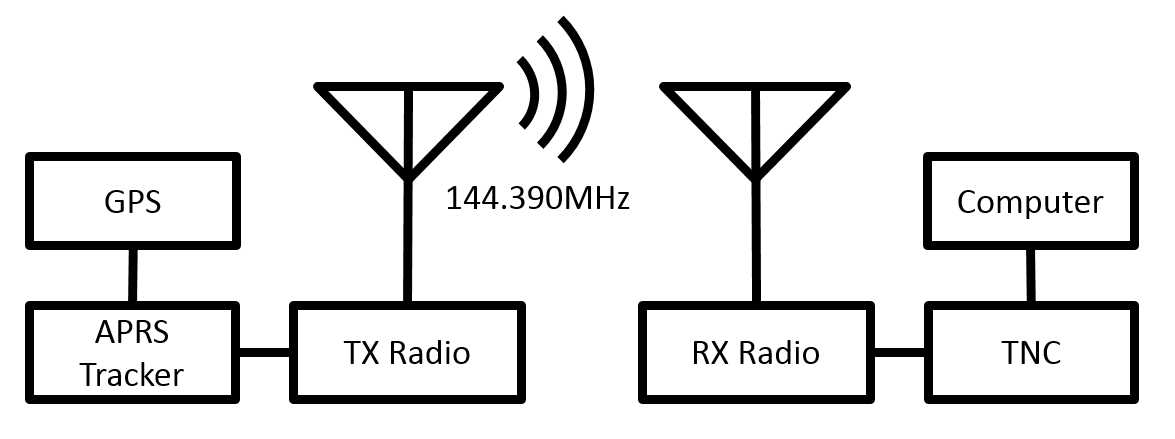
\includegraphics[width=0.75\linewidth]{images/APRSEndToEnd.PNG} 
   \caption[Block diagram of an example APRS system end to end.]{Block diagram of an example APRS system end to end. The GPS communicates information using NEMA to the APRS tracker, the tracker then takes this information and the preferences in its configuration to formulate APRS packets. The APRS packets are encoded by the tracker and the resulting audio passed to a transmit radio which sends the data. Typically this is done on frequency 144.390MHz in the United States. Receiving radios tuned to the same frequency pass the received audio to a TNC which decodes the packet and passes it to a computer using RS-232.}
   \label{APRSEndToEnd}
\end{figure}

The reasoning for trying to make improvements in software based demodulation are many, but a few of the more motivational ones are to follow. One advantage of doing software based demodulation is that it removes the necessity of specialty hardware; Instead of having dedicated hardware whose sole purpose is to modulate and demodulate APRS packets, hams can use a computer to do these tasks. By using a computer's sound card, audio from the radio can be processed using software to decode received packets, or audio can be played from the sound card to the radio to be transmitted. With the abundance of personal computers, this can provide a much cheaper solution for hams who are interested in trying out APRS without having to put down a potentially big initial investment (\textasciitilde\$200\,\cite{Kantronics2014,Outlet2014}) for a piece of hardware that serves one purpose. The price of this specialty hardware is steep and it is limited to only performing communication on a single channel. When using a line in / out on a computer they are typically stereo, meaning that a single sound card could handle operations on multiple channels. If two channels just is not enough the capabilities of a computer demodulator can be expanded by merely adding another sound card which is relatively cheap at \textasciitilde\$20\,\cite{Newegg}. See Table \ref{costCompareTable} for a comparison of the cost for hardware and software. From the table it can be seen that the cost to perform communication on 4 channels using dedicated hardware the cost would be \$800! For this cost a whole computer with a half dozen sound cards could be purchased, only further expanding capabilities.

\begin{table}
	\begin{center}
		\begin{tabular}{ | l | r | r | r | r | }
		\hline
			Cost for: & 1 Channel & 2 Channels & 3 Channels & 4 Channels \\ \hline
			Software & \$0 & \$0 & \$20 & \$20 \\ \hline
			Hardware & \$200 & \$400 & \$600 & \$800 \\
			\hline
		\end{tabular}
		\caption[Hardware and Software Cost Comparison]{Cost comparison of conducting APRS communications on 1 through 4 channels for hardware versus software assuming the user already owns a computer.}
		\label{costCompareTable}
	\end{center}
\end{table}

In addition to the the price advantages of software based demodulation approaches, there is also one other primary advantage. If software is being used instead of hardware there is the potential for a lot more capabilities since processing power and available memory increase drastically. For instance, one of the dedicated hardware solutions, the Kantronics KPC-3 Plus, has a mere 512KB of memory compared to that of any computer which is over 4GB as of 2014 - and that is just the ram, not hard drive space\,\cite{Kantronics2014,Graham-Smith2014}. Additionally, instead of just being able to handle live events and process each data point in the best manner possible as soon as it comes in, post processing becomes an option.

With the cost and versatility of a software demodulation solution now introduced, the paper addresses the following: Chapter 2 goes into background information, with a deeper introduction to APRS and a presentation of the aspects important to understanding this research. In Chapter 3, some of the current methods for interfacing with APRS, both hardware and software, are explained. Demodulation techniques are discussed in Chapter 4. Chapter 5 talks about the challenges of demodulating APRS packets. Chapter 6 discusses the methods used for benchmarking and comparing the demodulators. In Chapter 7, information on how the demodulators and algorithms are tested is presented. Chapter 8 goes into more detail about the software implementations in this project. Chapter 9 discusses the results of both the newly implemented algorithms and compares them to other demodulators. Areas of additional research and future work are discussed in Chapter 10. Chapter 11 is concluding remarks.

\chapter{APRS Background and Definitions}
From the introduction it is known that APRS is a method of digital communication used by hams in order to inform other hams of their location. In addition to supporting sending positions, APRS can be used to send messages, bulletins, weather, and other information. Since these packets are transmitted via radio  - which has limited coverage - APRS can be viewed as a local area awareness network. This gives hams who are listening for and decoding APRS packets information about nearby transmitting stations. This brief overview should give a little insight into APRS, but the rest of the section will focus more on what is going on behind-the-scenes to explain how APRS works in terms of the protocols, data transmission, modulation, etc.

In order to organize this discussion of the different components of APRS let us break it down into the Open Systems Interconnection (OSI) model representation. However, before fitting it into the OSI model here is a brief reminder of the relevant layers that are going to be discussed. Layer 1 of the OSI model is the physical layer. The physical layer consists of everything that is used to transport one bit of information from one location to another. The second layer is the data link layer. Within the data link layer bits from the physical layer are passed up to the network layer, and information from the network layers is framed and handed off to the physical layer. Layer 3 is the Networking layers. This Layer is responsible for determining the path that packets will take and providing flow control to prevent flooding. Above these layers are layers 4-7 which are the transport, session, presentation, and application layers respectively \cite{Sosinsky2009}. These upper layers get too inter-tangled to be able to cleanly separate them. For instance within the AX.25 2.2 specification a TNC is mentioned that only implements layers 1, 2, and 7 of the OSI model \cite{Beech1998}.

Here is the best division of APRS into the OSI model, following introducing this division each layer will be individually discussed in more detail. Layer 3 of the OSI model for APRS is the the AX.25 Protocol,  High-Level Data Link Control (HDLC) protocol composes layer 2. All the way at the bottom, layer 1 for APRS consists of the Terminal Node Controller (TNC) and Radio \cite{Silver2013}. A brief note on why the discussion begins with Layer 3 is because this is how the data is transferred. The interest stop here and does not continue to the layers above layer three, because those are all application specific. Starting with AX.25 the background information will be given down to Layer 1 which is where this research actually aims to make a contribution.

\section{Layer 3 - AX.25}
Layer 3, the network layer, is responsible for routing frames between individual nodes in the network. A frame of data is more traditionally called a packet at this point since AX.25 is a packet switched network protocol \cite{Peterson2011}. AX.25 is the amateur X.25 protocol. Meaning that the AX.25 protocol, which is what APRS uses, was developed my Amateur radio operators and is based off of the x.25 protocol. Since the origins of AX.25 lie within X.25, the discussion will begin with X.25. 

\subsection{X.25}
Developed in the 1970s the packet switching protocol X.25 was deployed on telephone networks where it was used until it began to be displaced by the IP protocol. The X.25 protocol suite provides OSI layers 1-3, although it does have standards that support each of those layers \cite{Sosinsky2009}. For instance the X.21 standard is commonly used for layer 1 of X.25 and ISO 7776 specifies a Link Access Procedure Balanced (LAPB) to assists with layer 2, the data link layer \cite{Gallagher1997}. The Data Link layer of LAPB, a bit oriented protocol derived of HDLC,  manages packet framing and ensures that frames are error free and properly sequenced. When used on telephone networks there were five distinct modes that the protocol would operate in: Call setup for establishing the connection, Data transfer, idle where the connection is established but no data is being transferred, call clearing for terminating the connection, and restart for resynchronizing the host and client \cite{Javvin2006}. Many of the features of the Layer 2 and Layer 3 operations of X.25 can be found in at least a similar fashion in AX.25.

\subsection{AX.25}
Next the AX.25 protocol will be discussed through comparison and contrast with X.25. One of the main differences between the X.25 and AX.25 is that when the specification is read, in addition to specifying the behavior of Layer 3, the behavior of Layer 2 is also included. Although this is somewhat implied for X.25, there are still separate documents for the specifications for each one of the layers. After reading the specification for AX.25 it very clearly defines the framing with starting and terminating flags as well as the networking and routing \cite{Beech1998}.

\section{Layer 2 - High-Level Data Link Control}
The goal of HDLC is to make sure that when the data is received and passed up to Layer 3, that it is error free, without loss, and in the correct order \cite{Javvin2006}. There are a few ways that HDLC accomplishes this, two of which are framing and with the Frame Check Sequence (FCS). The framing occurs through the use of flags around the data. A flag is one byte and is hex 0x7E. For APRS common practice is to send multiple flags consecutively to give transmitting radio time to key up and settle or to give receiving radios time for their squelch to open. Since it is an non-return to zero inverted (NRZI) encoding no change in frequency corresponds to a 1 and a change in frequency corresponds to a 0. As such multiple 1s in a row make it hard to keep timing which is why bit stuffing is used. With the exception of the flag which contains six consecutive 1s (01111110) if there six or more consecutive 1s in the data packet a zero will be stuffed after the fifth 1 to increase the clocking energy in the signal.

\section{Layer 1 - The Bell 202 Modulation and the Radio}
Since Layer one is composed of the things needed in order to transmit one bit from one location to another, it needs to be made clear what all this includes for APRS. Starting with air, the medium through which the radio frequency (RF) signals propagate, the RF transmissions are received or transmitted by the radio. Without decomposing the radio into all of its individual components, the audio that the radio receives then has to be processed. In order to stay focused on what happens in layer 1 and not start mixing the other layers together some more discussion of what this audio signal consists of is necessary.

The audio signal that contains the APRS packets is composed using the Bell 202 modulation which is an Audio Frequency Shift Keying (AFSK) mode. As such RF either comes in through the radio, is translated to the corresponding audio, and then demodulated into a bit stream by interpreting the Bell 202 modulation. Or, a bit stream from layer 2 of APRS is modulated using the Bell 202 modulation, this modulated audio is passed to the radio, and the radio then transmits it out. Since decomposing the radio down into its individual components does not have any affect on representing the different OSI layers of APRS, it will not be discussed. However there are factors that affect wireless communications and RF signals that will be discussed in chapter 4.

\subsection{Frequency Shift Keying}
In order to understand the Bell 202 modulation scheme the communication mode of AFSK needs to be introduced. AFSK is a form of frequency shift keying (FSK) that occurs by modulating frequencies in the audible range. FSK uses multiple frequencies in order to represent the different symbols such as 1 or 0 or mark and space in our case. If the frequency of the data carrying signal can be determined, then the symbol is knows for that bit period. FSK is the more generic term and is used for 9600 baud (bits per second) APRS on Ultra High Frequencies (UHF). In this mode the actual RF carrier in the 440MHz band is modulated between one frequency and another nearby frequency in order to represent the two different symbols. In contrast, AFSK switches between two different audio signals, which for APRS on Very High Frequencies (VHF) is then modulated onto the RF carrier using Frequency Modulation (FM).


\subsection{Bell 202}
With FSK and AFSK now introduced the AFSK used within Bell 202 can be described. The Bell 202 modem was patented in 1984 using 1200Hz and 2200Hz tones, although the patent was originally filed in 1981 \cite{stauffer1984fsk}. Interestingly, the International Telecommunication Union (ITU) did not publish a standard for this modulation that were used in telephone networks until 1988. In the standard, however they use 1300Hz tone for symbol 1 and 2100Hz tone for symbol 2 called a mark and space respectively \cite{ITUV23}. The original bit stream is modulated using a non-return to zero inverted (NRZI) encoding. This means that when a transition occurs from one symbol to another in the Bell 202 modulated signal this symbolizes a 0 bit in the original data bit stream and if the Bell 202 symbol remains constant over multiple symbol periods, that signifies a 1 bit in the original data bit stream. For Bell 202 the frequencies that are used are 1200Hz and 2200Hz tones for the mark and the space as opposed to the 1300Hz and 2100Hz tones proposed in the ITU specification.

\chapter{Approaches to Accessing the APRS Network}
In the world of APRS, there are many solutions that hams take advantage of in order to utilize the network. Some they find and make work, some they purchase to use exclusively for APRS, and some go through the trouble of building their own solutions. This chapter explains some of the common systems used on the APRS network, primarily those that can be used for receiving, starting with terminal node controllers and progressing to software based demodulation.

\section{Terminal Node Controllers}
Currently there are many systems that will demodulate Bell 202 encoded APRS packets. The original hardware used for this communication style was dedicated modems similar to dial-up 56k modems that did the encoding and decoding. These modems were connected directly to the radio and the would decode the signal that the radio received as well as sending audio to the radio to transmit. Virtually identically, the terminal node controller (TNC), a specialized modem used in APRS operation, signals the radio to transmit when it has data to send out and decodes received radio audio\,\cite{Wolfgang2005}. A reminder of the age of the technologies that are being used for the data transport of APRS, packet radio originated in the 1980s as TNCs became affordable\,\cite{Helms1992}. This means that this technology is over 30 years old at the time of writing in the year 2016.

With a radio and a TNC, amateur packet stations and digipeaters (digital packet repeaters) are possible\,\cite{Group2012,Wiki2012}. Digipeaters are an essential part of the ham packet network, but many users wish to report their GPS position onto the APRS network instead of just relaying traffic for other stations. In order to accomplish this, a GPS receiver is required. Now, stations can take the data from their GPS receiver and put it in the payload of the APRS packet and transmit the GPS position onto the network. One other common use of a TNC is an Internet attached digipeater, usually though the use of a computer, that would allow the data to be posted to the APRS-IS servers\,\cite{Community2015}. To give an example of some of the TNCs available, those within the testing testing scope of this project will be listed. There are a total of eight TNCs - six unique models - whose decoding results are compared to the software approaches. These modems included two Kantronics KAM Plus, a Kantronics KAM, an MFJ-1278, two AEA PK-88, a PK-232, and a PK-232MBX. An example image of what a TNC looks like can be seen in Figure \ref{kantronicsKamPlus}.

\begin{figure}
  \centering
	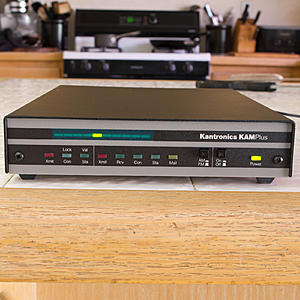
\includegraphics[width=0.75\linewidth]{images/Kantronics-KAM-Plus.jpg} 
	\caption{Image of the Kantronics KAM Plus TNC\,\cite{KK6RF}.}
   \label{kantronicsKamPlus}
\end{figure}

\section{Specialized APRS Hardware}
Many people know exactly what they would like to do with APRS and exactly what traffic they want to contribute to the APRS network. So, instead of purchasing an expensive Multi-mode TNC, companies are making dedicated APRS solutions available to consumers for a fraction of the price. In addition to making this hardware available, the producers support the hardware and make pretty user interfaces for the users to be able to program the hardware exactly as they like and without having to invest much time into understanding how different components work together. Some examples of APRS exclusive devices are Argent Data's OpenTrackers (Figure \ref{openTracker3}), Byonics' TinyTrack, and Fox Delta's Fox Track\,\cite{Miller,Byonics,Foxtrak}. These compact packages along with a radio and a GPS module perform APRS tasks at a satisfactory level for many users.

\begin{figure}
  \centering
	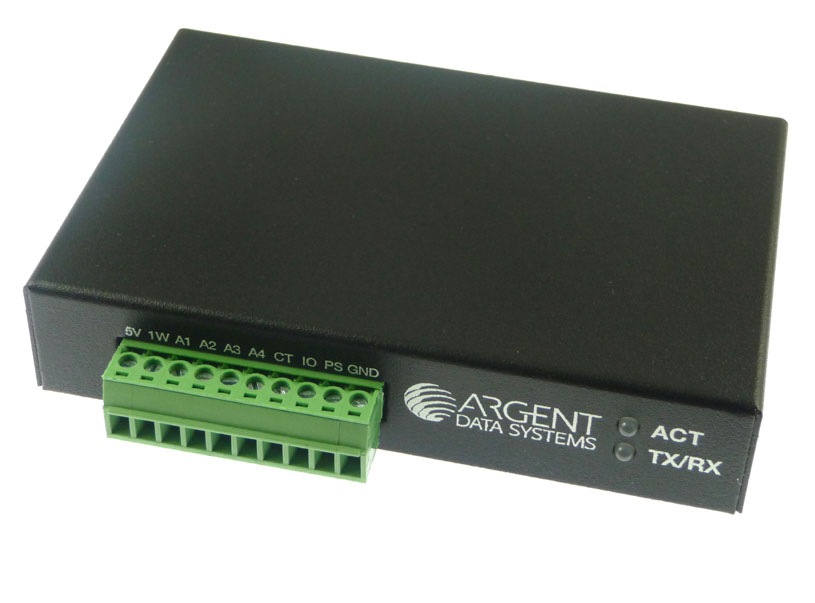
\includegraphics[width=0.75\linewidth]{images/Ot3m-termblk.jpg} 
	\caption{Image of Argent Data's OpenTracker 3\,\cite{Data}.}
   \label{openTracker3}
\end{figure}

Since the average user only wants to report positional information, these dedicated devices are simple to setup to do such tasks, but include only a simple feature set. Although these trackers contain some features, since they are all small embedded systems they cannot and do not have implemented all of the features that APRS supports. An example is the messaging service; since these devices do not have a display or a keypad, there is no way to input or display a message. Certain radio manufacturers have begun integrating the TNCs into the radios themselves to utilize the radio�s screen. The Kenwood TM-D700 series and Yaesu FTM-350 (Figure \ref{yaesuFTM350}) are examples\,\cite{Kenwood,Yaesu}.

\begin{figure}
  \centering
	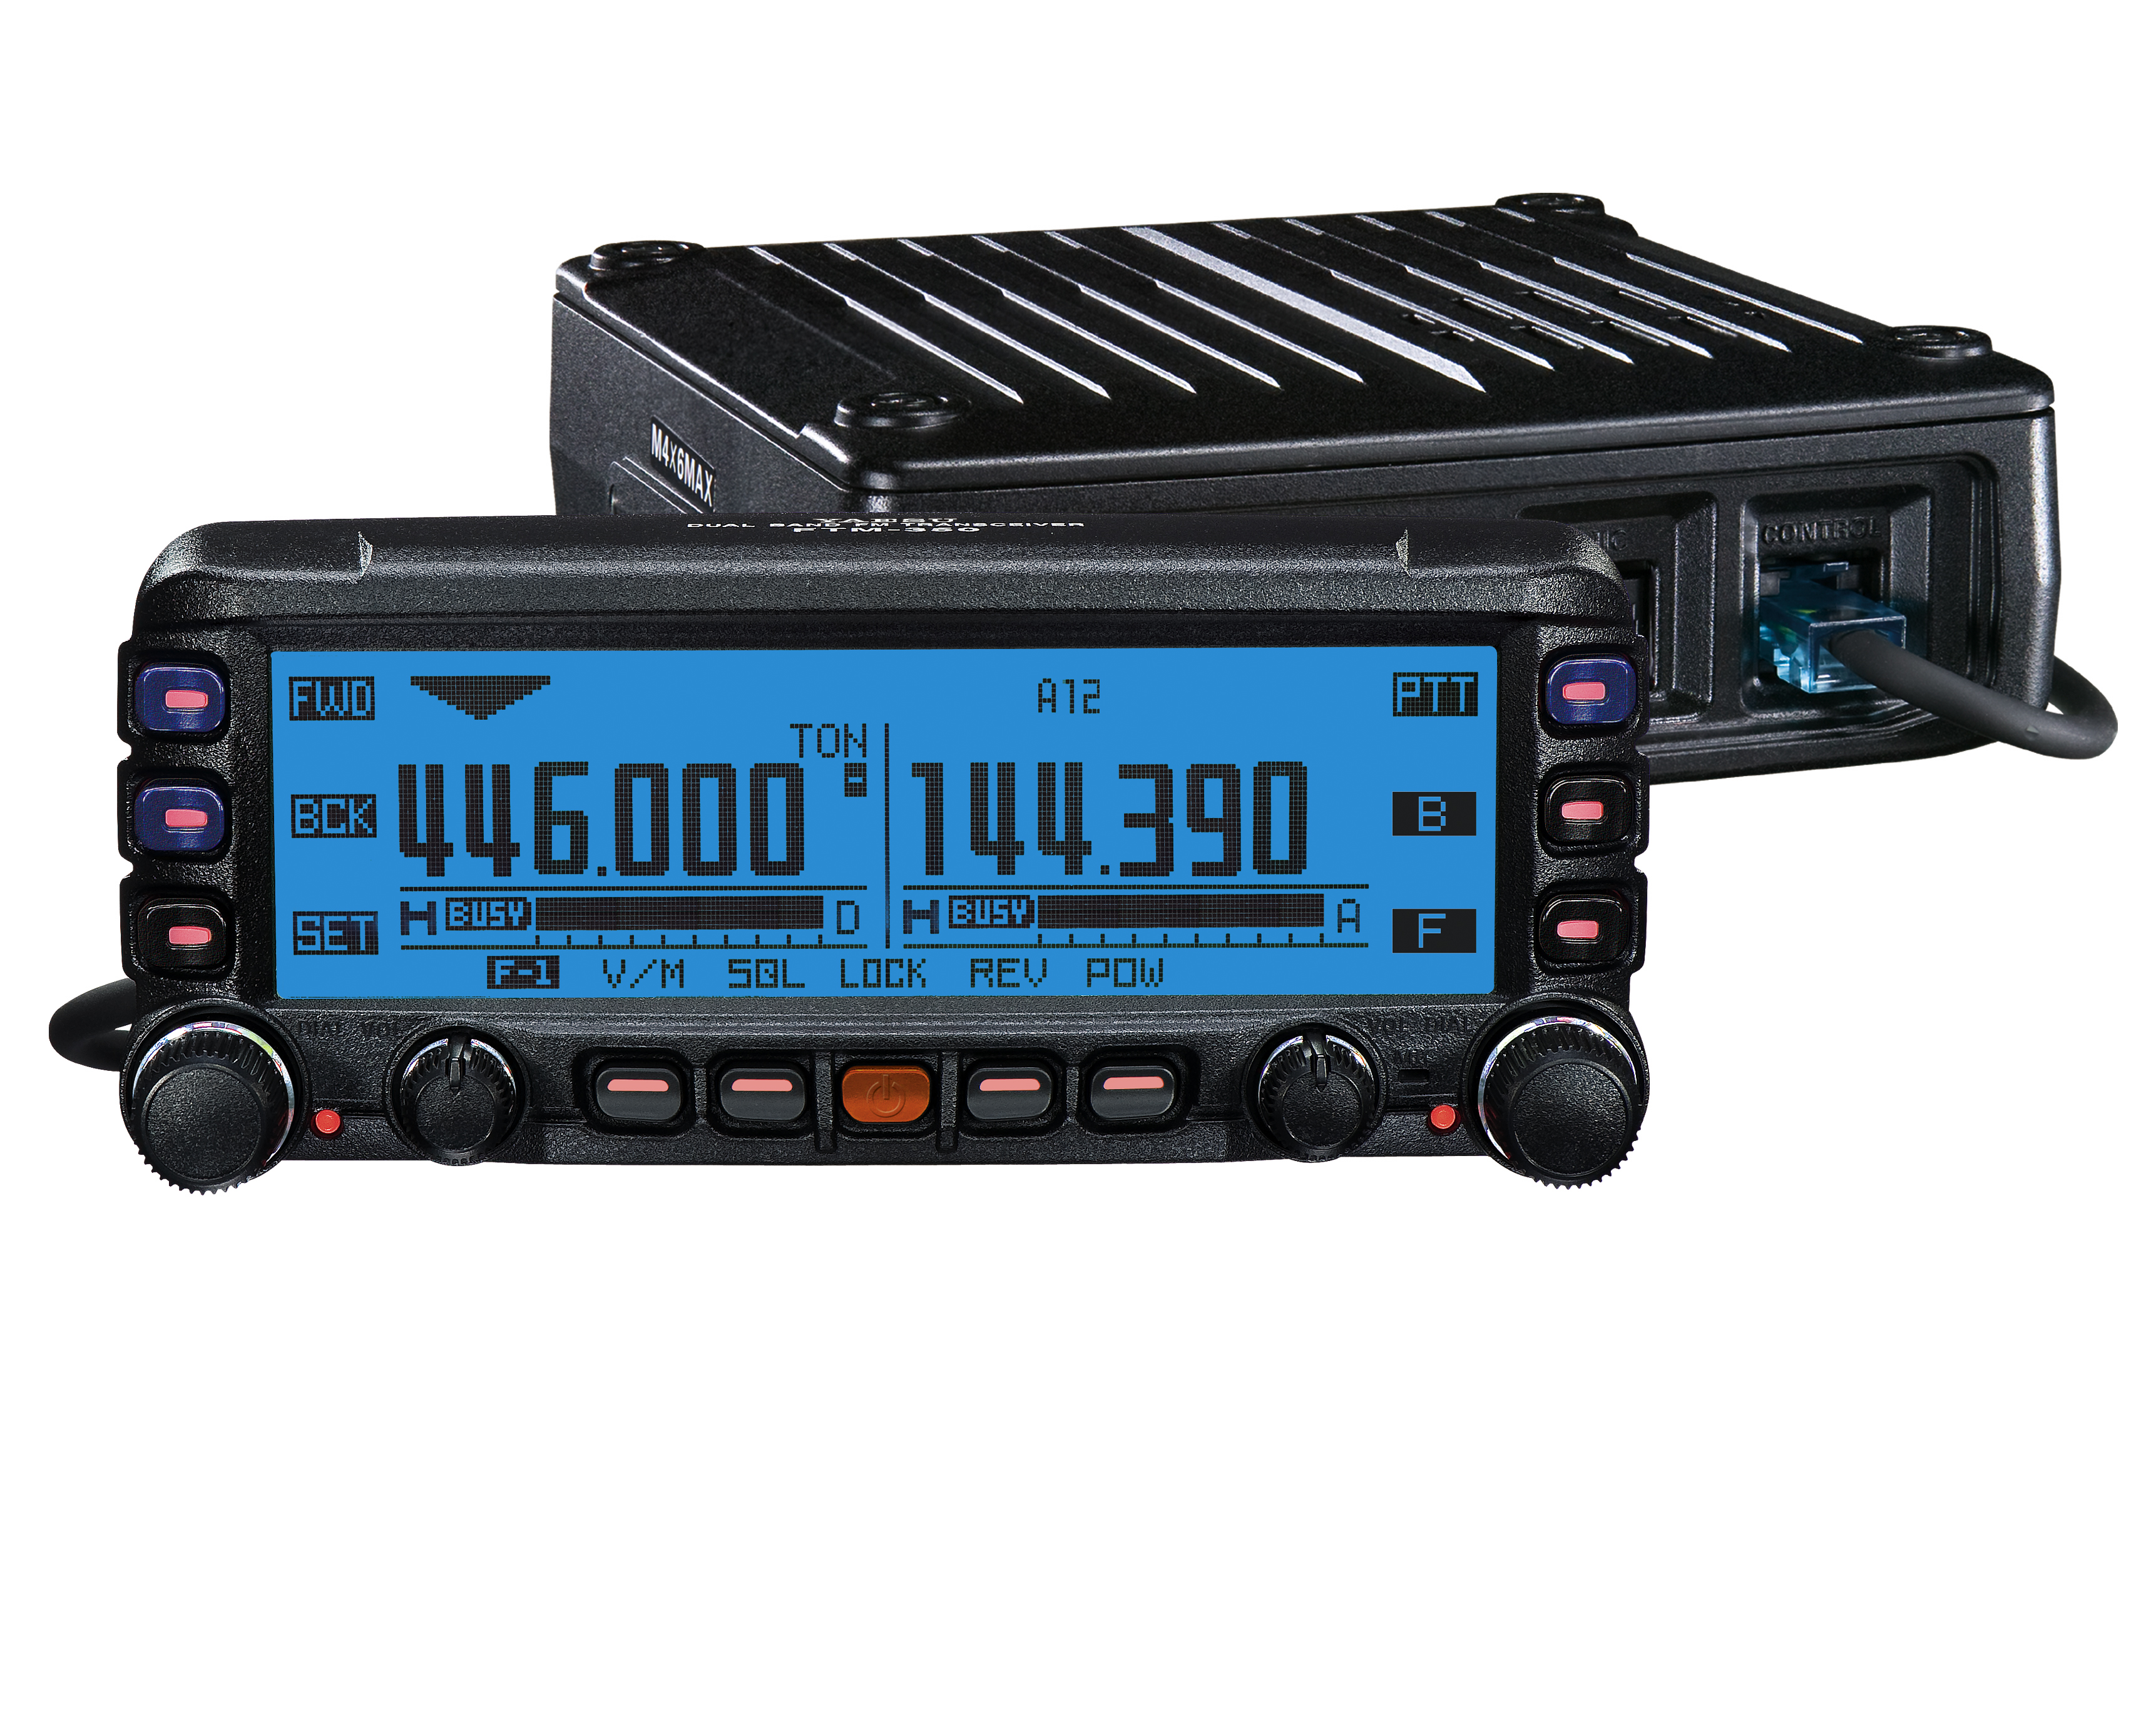
\includegraphics[width=0.75\linewidth]{images/FTM-350US_F.jpg} 
	\caption{Image of the Yaesu FTM-350 Radio which has APRS integrated\,\cite{Yaesua}.}
   \label{yaesuFTM350}
\end{figure}

However, both the options in this section and the one previous on TNCs require going out and buying special hardware in order to utilize APRS. This can be expensive and cost prohibitive for some hams to be able to begin APRS operations.

\section{Software Based Demodulation}
It's fair to assume that before a ham operator becomes interested in the APRS network and sending APRS packets that they will already have a radio. So, if they already have a radio all they have to do is buy a piece of hardware that will do the modulation in order to send a packet. However, hardware costs money and before diving right in, some users might appreciate being able to try APRS out first. A good, cheap alternative to dedicated hardware is to use hardware that hams already have. A good choice that will fit the needs is a computer, which most hams are likely to already own. If they don't happen to own a computer, much of this argument is null and void since a computer is required to use both TNCs and to program the specialty hardware. On the computer amateurs can use software to do the modulation and demodulation, and build or buy a cheap interface to a radio, around \$15 instead of roughly \$150 for a piece of dedicated hardware.

This seems to be a route that some are taking and a demodulation scheme that this project explores in detail, but before exploring this in more detail, more information on current systems that operate in this software realm is necessary. Some examples of the software that can be used are George Rossopoylos's Packet Engine\,\cite{Rossopoylos}, Thomas Sailer's Linux Sound Modem\,\cite{Sailer1997,Sailer2000}, and Sivan Toledo's JavaAX25\,\cite{javax25github, Toledo2012a}. On a computer, even one with minimal resources, there are algorithms that are being used to demodulate the APRS packets. Again, what this project aims to investigate is what improvements can be made to the algorithms and software-based demodulation approaches in order to decode these packets in a more robust fashion and to try and get similar performance to TNCs and dedicated hardware. Based on observations in initial analyses where software was unable to decode packets, the hypothesis is made that improvements can be made to software based demodulation.

\subsection{javAX25}
Sivan Toledo's javAX25 is one method of utilizing the APRS network. Toledo's software is very comprehensive in handling the encoding, decoding, radio control, and interfacing with sound cards to allow for full use of APRS. However, in addition to just being able to utilize APRS, there is also a test application inside of this package that allows for quick and easy testing of everything in the suite - of the most interest, however, is the ability to test demodulators. Although all of these features were included, the three primarily used in this project were the modulation, demodulation, and demodulator testing. Due to its comprehensiveness and ease of access online through Github, javAX25 was chosen to be the basis for this project\,\cite{javax25github}. For a complete list of features the manual can be found in the following reference, and even from the beginning the mission statement he outlines coincides with that of this research\,\cite{Toledo2012a}.

Toledo did some benchmarking of his software and found that running two demodulators in parallel provided the best results. The demodulators were exactly the same; the only difference was that one was processing data after a bandpass filter that was centered around the two frequencies of interest, and the other had a bandpass filter that in additionally applied 6dB of attenuation at 1200Hz\,\cite{Toledo2012}. Being published in 2012, this is the newest reference in this paper on the subject of AX.25 (aside from the papers published by Finnegan), which provided additional incentive to use this project for this research. As added verification of making the correct decision of what software to use, a very popular Android APRS application written by Georg Lukas uses javAX25 by a direct import\,\cite{APRSdroid}.
\chapter{Bell 202 Demodulation Techniques}
There are a few primary approaches to demodulating 1200 baud 1200Hz/2200Hz AFSK signals in hardware.  However, before talking about the techniques for doing AFSK demodulation, it is worth specifying what type of FSK Bell 202 is. There are two features that are relevant for taking into consideration when demodulating the signal. First is that it is asynchronous, meaning that there is no separate clocking signal as the clocking is embedded within the data signal, hence the conversation on bit stuffing and clocking energy in the APRS Background chapter. If it were synchronous, there would be two different signals coming into the demodulator (which would be the data carrying signal and a clocking signal). The second characteristic is that the FSK is coherent or continuous. This means that there is a continuous signal at bit boundaries and there are no jumps as the signal changes from one frequency to another as seen in Figure \ref{coherentFSKExample} as opposed to non-coherent Figure \ref{noncoherentFSKExample} which does have these jumps. Another name sometime applied to this method of FSK, coherent FSK, is continuous-phase frequency shift keying or CPFSK\,\cite{WikipediaCPFSK}.

\begin{figure}
	\centering
	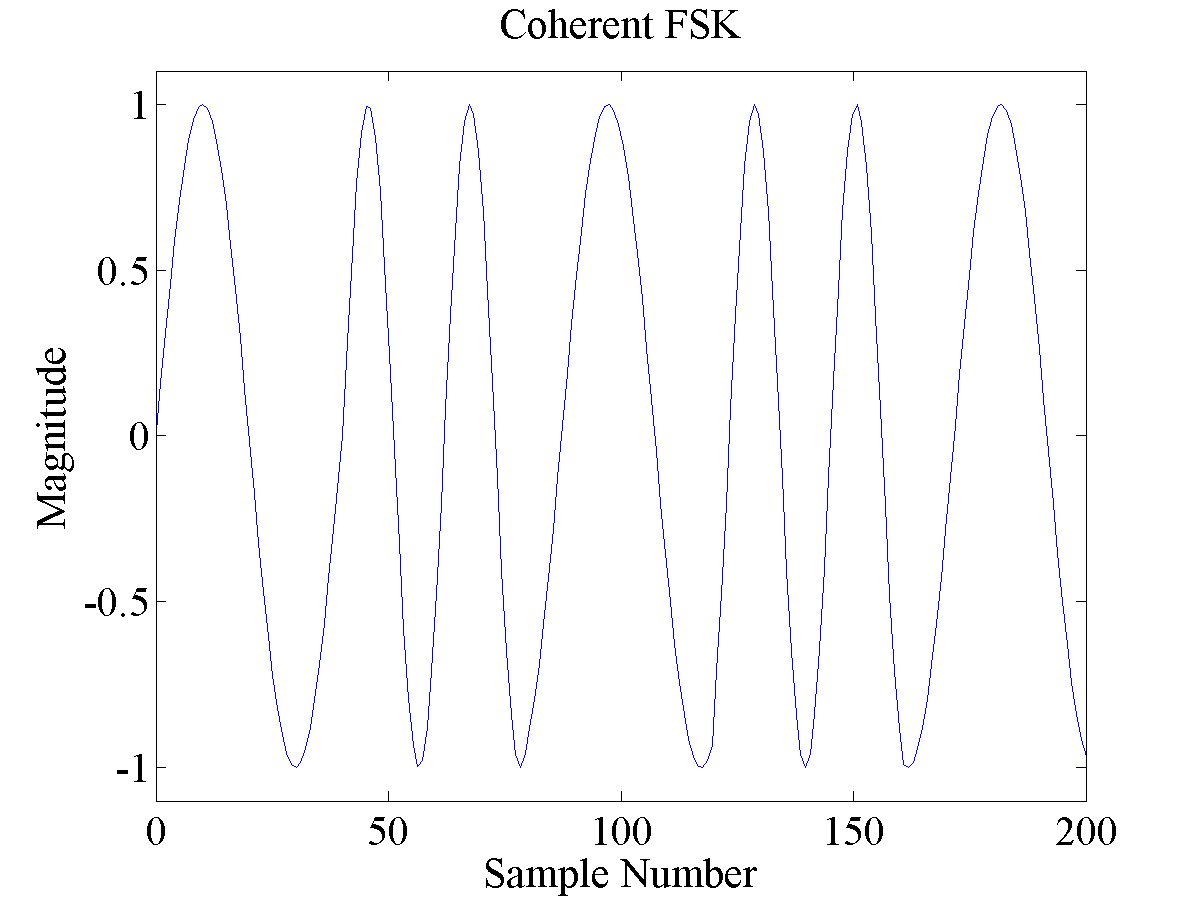
\includegraphics[width=0.75\linewidth]{images/CoherentFSK.png} 
	\caption{Example of a coherent FSK signal.}
	\label{coherentFSKExample}
	\vspace{15mm}
	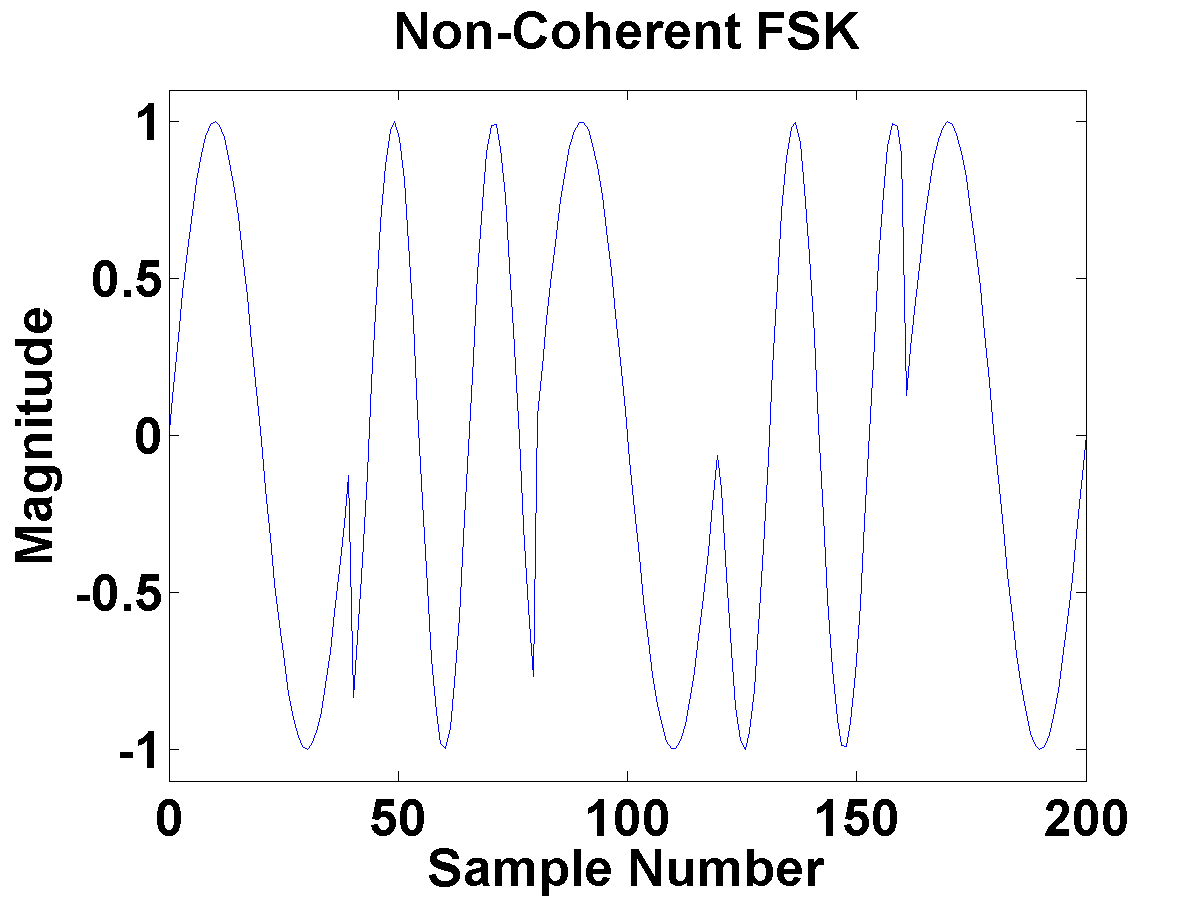
\includegraphics[width=0.75\linewidth]{images/NonCoherentFSK.png} 
	\caption{Example of a non-coherent FSK signal.}
	\label{noncoherentFSKExample}
\end{figure}

Among the demodulation techniques for coherent FSK are edge detection, correlation, filtering, and phase-locked-loops (PLLs). Each of these will be explained in more detail in the corresponding sections below; however with Correlation and Filtering being very popular and mentioned in many books and applications, there is a lot of overlap so more detailed information can be found in the following references\,\cite{MarvinK.Simon1995,Sklar1988,J.Das1986,Proakis1983,Seguine2006,Semiconductor}. The following sections in this chapter explain how the demodulation approach works with the software implementation details being saved for the Implementation chapter. However, there will be an additional section at the end of this chapter to discuss some of the potential advantages of using software over hardware. Before talking about all of the techniques a little context as to which onces are being used in the various pieces of harwadware can be found in Table \ref{HardwareDemodTechniques}.

\begin{table}
	\begin{center}
		\begin{tabular}{ | l | l | }
			Device & Demodulation Technique \\ \hline
			OpenTracker 2 & PLL using XR-2211 \\ \hline
			OpenTracker 3 & Software time delay correlation \\ \hline
			Kantronics Kam & Edge detection using TCM3105 Chip \\ \hline
			MFJ-1278 & PLL using XR-2211 \\ \hline
			PK-88 & Digital filters using AMD 7910 chip \\ \hline
			PK-232 & Analog filters \\ \hline
		\end{tabular}
		\caption{Hardware Demodulation Techniques. \cite{Inc.2001,EXAR1997,Devices1989,Instruments1994,MFJ1278Man,PK88Man}}
		\label{HardwareDemodTechniques}
	\end{center}
\end{table}

\section{Edge Detection}
An edge detection, or zero-crossing, demodulator identifies rising and falling edges in the signal to determine the frequency present. In the TCM3105 chip, which is an FSK modem, rising and falling edges trigger pulses that are at a frequency that is double the input frequency\,\cite{Instruments1994}. Although this is how it is done in hardware, it may be easier to understand through the more simple discussion of zero-crossings. The idea is that based off of the time elapsed between zero crossings (rising and falling edges or vice versa) of the signal, one-half the period of the waveform can be measured. Once the period has been measured the frequency can then be easily calculated using the inverse relationship between period and frequency, \textit{f} = 1 /T where \textit{f} is the frequency and T is the period\,\cite{Seguine2006}. Just to reiterate, two consecutive zero crossings is only half of the period do to the nature of sinusoidal signals. As the TCM3105 is an older chip, a replacement is now commonly used in 1200 baud modem projects, and that is the MX614 made by MX-COM\,\cite{Mitrenga2000}.

\section{Correlation}
A correlation demodulator works through correlating - comparing - an FSK signal with the possible options based off the modulation scheme. In this instance we expect the signal to be either a 1200Hz or 2200Hz signal and hence the signal will be compared to two internal oscillators, one at each frequency\,\cite{Rowe2014}. In practice, the input signal is mixed with each one of the two reference signals and then integrated. The results from each of these correlations is then fed into a decision unit. The output of the decision unit is whichever of the frequencies has more power and hence was more prominent in the signal. The basic block diagram can be seen in Figure \ref{BlockDiagrams}. Correlation is the current method used in Toledo's javAX25. An alternative implementation of a correlator is to have a delay line instead of an internal oscillator. This delay line can delay the input by the time for one period of an expected frequency (i.e. 1/2200Hz) to elapse and then this delayed signal can be multiplied by the original signal\,\cite{Seguine2006}. Essentially, the delayed signal becomes the internal oscillator in this example (see Figure \ref{TimeDelayCorrelator}). Side note, this would work better for higher frequencies than those here since the delay line would be about 145 miles long if using copper wire for the 1200Hz tone\,\cite{HowFastIsElectricity}.

\begin{figure}
  \centering
	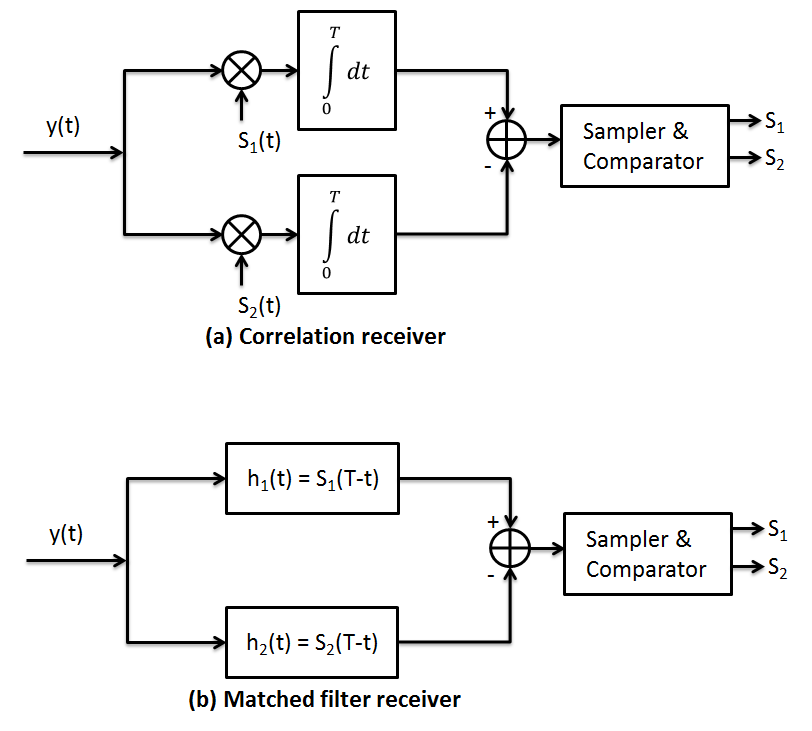
\includegraphics[width=0.75\linewidth]{images/MyBlockDiagrams.png} 
	\caption{Block diagrams for (a) A Correlation Receiver and (b) A Matched Filter Receiver\,\cite{J.Das1986}.}
   \label{BlockDiagrams}
\end{figure}

\begin{figure}
  \centering
	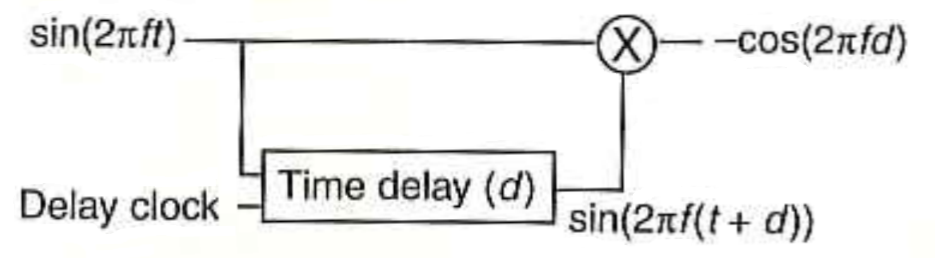
\includegraphics[width=0.75\linewidth]{images/TimeDelayCorrelator.png} 
	\caption{Block Diagram of a time delay correlator\,\cite{Seguine2006}.}
   \label{TimeDelayCorrelator}
\end{figure}

\section{Filtering}
Much like the correlation demodulation approach, a filter based demodulator operates on knowing the expected frequencies in the FSK signal. For our case of 1200Hz and 2200Hz frequencies, a filter will be set and centered about each one of these frequencies. The input signal is passed to each one of these narrow band pass filters and then the power of each of the signals out of the filters is fed to a comparator. The stronger of the two frequencies is the one that must have been present in the original signal\,\cite{Watson1980}. One example of a filter that can be used is a Finite Impulse Response (FIR) Filter. The block diagram for this approach can be seen in Figure \ref{BlockDiagrams}, and the general structure is very similar to correlation. This method seems to be prevalent in both hardware and software based approaches. For instance, if one examines the schematic for the PK-232 MBX, two parallel filters can be seen\,\cite{Inc.2001}. Rossopoulos's Packet Engine measures the energy on the two modem frequencies using filters to do the demodulation. Sailer's Sound Modem also uses a matched filter demodulation\,\cite{Sailer1995} whose algorithm was then reused on a micro controller by Holder\,\cite{Holder2012}. Additionally, AMD produced an FSK Modem chip that used digital filtering for demodulation\,\cite{Devices1989}. All of these independent uses make this look like the most prominent approach for demodulation.

\subsection{Discrete Fourier Transform}
One example of a digital filter is a Discrete Fourier Transform (DFT). A discrete Fourier Transform is one implementation of Fourier Transform that is executed on discrete samples similar to what is present in a digital audio file. Once a Fourier transform has been applied on a signal the output is a relative power versus frequency. With this data, whichever frequency (either 1200Hz or 2200Hz) is more prominent is the symbol which must be present in the bit period, and hence can be used for the demodulation; however, Fourier Transforms are computationally intensive.

\subsection{Goertzel Algorithm}
Computing a discrete Fourier transform is more reasonable computationally than a full Fourier transform, which is a continuous integral as opposed to having discrete terms\,\cite{WikipediaFT}. However, even the results from the DFT have more data than is needed to do the demodulation since the results will be a spectrum of powers over a range of frequencies\,\cite{WikipediaDFT,WikipediaFFT}. A more simplified and specific approach can be used. The Goertzel Algorithm evaluates the coefficients and corresponding powers of the individual frequencies of 1200Hz and 2200Hz\,\cite{WikipediaGA,Elmenreich2011}. This approach, sometimes called a Goertzel Filter, means that no additional computation is wasted on computing frequency power data that is not relevant, making it faster and a vast simplification to the DFT\,\cite{SanjitK1993}.

\section{Phase Locked Loop}
Another option for determining the frequencies present in the original data carrying signal, and hence the actual data in the signal, is to use a Phase-Locked Loop (PLL)\,\cite{Akoum,Perrott2009,Lutus2011}. There are a few different approaches for utilizing a phase locked loop. The basic idea is that there is an internal oscillator and the input (the received signal) is used to influence this oscillator\,\cite{Gaeddert2013} . The input signal and the reference oscillator signal are integrated and this output is used for feedback to the internal oscillator (hence the loop portion of PLL)\,\cite{Roppel}. The convenient thing about monitoring the phase of the signal so closely and being able to stay locked onto it is that the frequency must also be known and this is the portion that is really of interest. A block diagram of a phase locked loop can be seen in Figure \ref{PLLBlockDiagram}. There is a chip produced by Exar that does FSK demodulation and tone detection using a PLL, for which the model number is XR-2211A\,\cite{EXAR1997}. A circuit diagram of using the XR-2211A for Bell 202 can be seen in Figure \ref{XR2211Circuit} which also shows some of the primary items needed for a PLL including the phase detection (integrator) and the VCO (Voltage Controlled Oscillator).

\begin{figure}
  \centering
	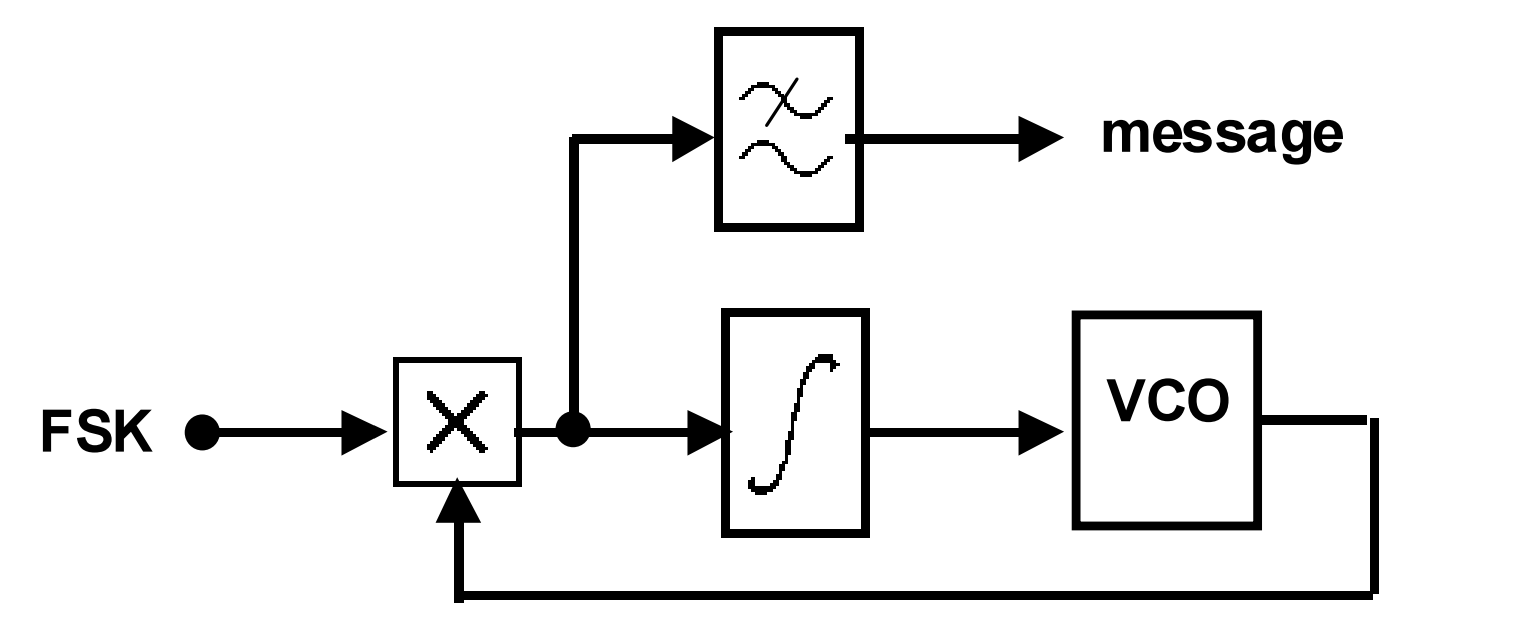
\includegraphics[width=0.75\linewidth]{images/PLLBlockDiagram.PNG} 
	\caption{Block diagram of a PLL demodulator\,\cite{Roppel}.}
   \label{PLLBlockDiagram}
\end{figure}
\begin{figure}
  \centering
	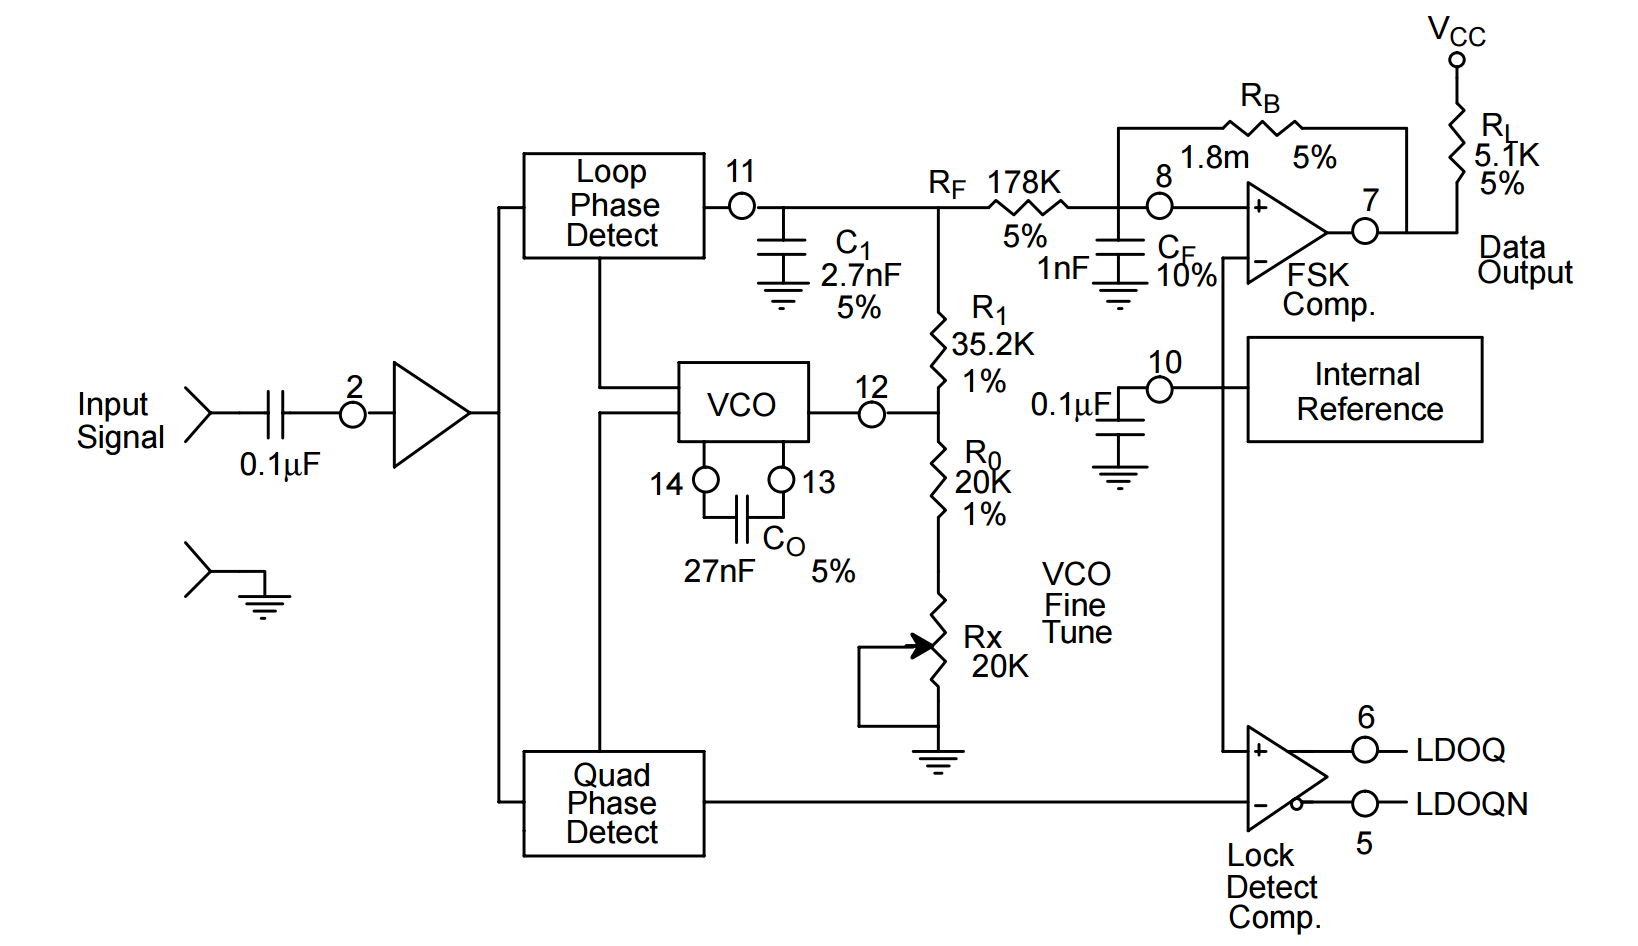
\includegraphics[width=0.75\linewidth]{images/XR2211Circuit.PNG} 
	\caption{Circuit connection for FSK Decoding of Bell 202 Format using an Exar XR-2211A\,\cite{EXAR1997}.}
   \label{XR2211Circuit}
\end{figure}

\section{Additional Benefits of Software Based Decoding}
Software is flexible. As Bergquist mentioned, it was only a matter of time before hams developed a bond between computers and radios using TNCs and it is time to take it a step further and leverage the capabilities of a computer even more\,\cite{Bergquist2001}. Any one of the aforementioned algorithms can be used on the same hardware without having to add additional discrete components, new Integrated Circuits (ICs), or make modifications to a Printed Circuit Board (PCB). There are two benefits of using software instead of dedicated hardware that this research will investigate; first exhaustive search of a signal through the use of buffers, and second, the ability to be able to run multiple of these demodulation approaches in parallel.

\subsection{Exhaustive Search of Incoming Signal}
Using software the input signal can be buffered in the program and then searched for a signal. Since there is not a separate data and clock signal, there could be a case when the clocking is improperly selected. Using an approach of buffering data that may contain a valid packet, the software can step through the data trying every possible clocking option.

\subsection{Taking Advantage of Parallel Demodulation}
Another advantage of using software for decoding these AFSK signals is being able to apply multiple demodulation techniques. Once the data is collected and converted to a digital form there is no reason, other than computation limitations of the host computer, not to run multiple algorithms in parallel in order to be able to demodulate the maximum number of packets possible. Although there are packets that every algorithm is able to decode, there are also packets that some approaches can decode while others can not. Through using multiple demodulators in parallel and de-duplicating the results, even more packets can be correctly decoded.

\chapter{Demodulation Challenges}
While analyzing different demodulation algorithms and trying to improve their performance, there were a few phenomena that were observed. Specifically, there were aspects that proved problematic for software based demodulation, and although they are probably challenges to all types of demodulation and not just those that are software based, they were noticed during these analyses. While inspecting performance of the algorithms the following items created difficulty and can all be attributed to the fact that APRS uses RF and hence is susceptible to all the items relating to an RF transmission. 

The main challenge in decoding the APRS data was the fact that the digital stream is converted to an audio signal and then transmitted over RF. The addition of RF adds a whole plethora of obstacles which can include Path Loss, Multi-path, Fading, Doppler effects, Co-channel interference, Interference and Noise, and Foliage \cite{Goleniewski2006}. A few items which are important to note, due to the fact that some of the algorithms had to be coded to tolerate them are: DC Offset, Noise, and Emphasis.

\section{Challenge: DC Offset}
An audio signal can be characterized by a sine wave. In order to get different sounds the frequency of the sine wave is changed and in the context here, the two frequencies are 1200Hz and 2200Hz. Since an audio signal is a sine wave, the average value should be zero. The zero value is commonly referred to as the ground of the audio signal, and as the definition would imply the signal should spend the same amount of time above ground as it does below ground. As the performance of zero crossing algorithms were investigated it was very evident that this was a challenge. If one assumes that the signal is centered about zero, and it is not, the logical decisions made with this incorrect assumption will hence not hold true. Figure \ref{DCOffsetExample} shows that the signal is not centered around zero. This lack of the signal being centered around 0 (or ground) is why it is said to have a DC offset. It can be noticed in this figure that near the center there are time periods that would be both much longer and much shorter than those expected from subsequent zero crossings during demodulation due to this DC offset effect.
\begin{figure}
  \centering
	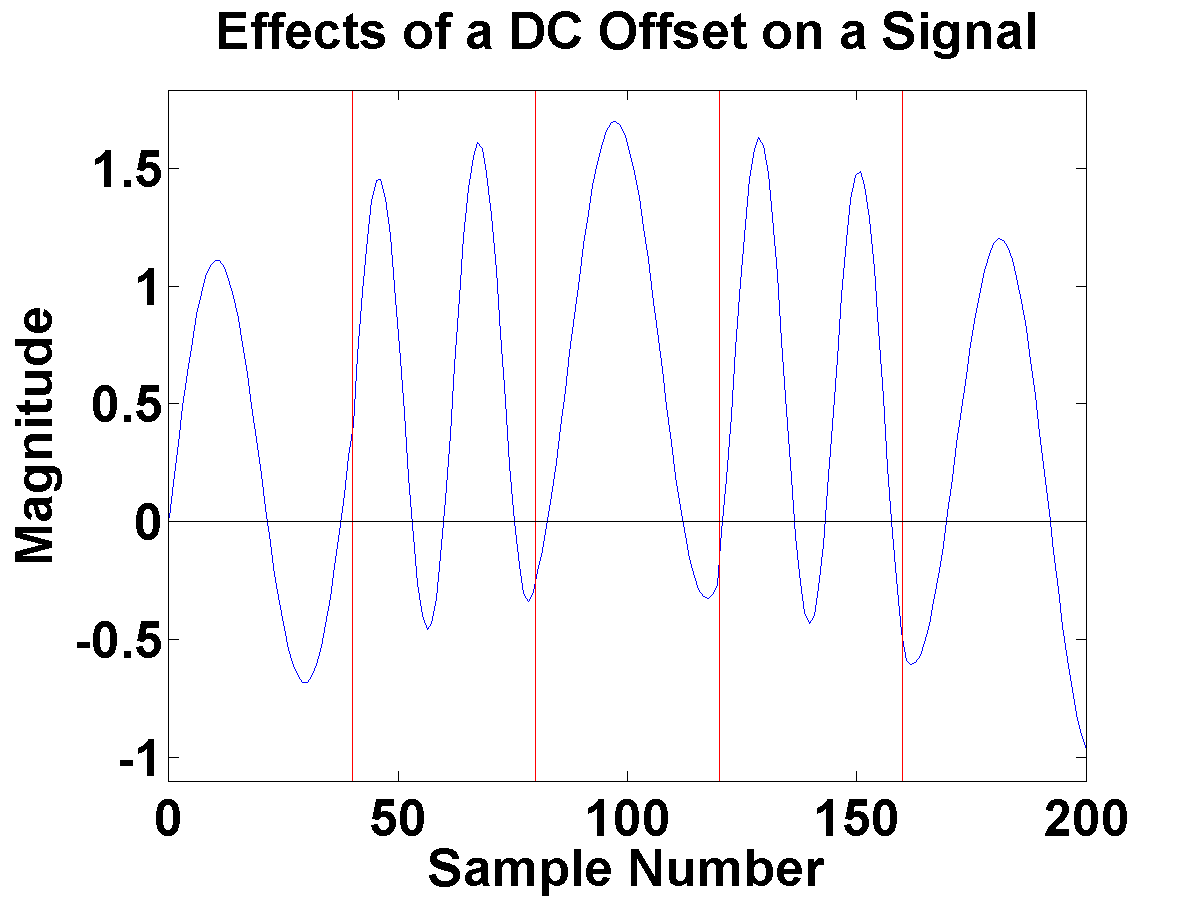
\includegraphics[width=0.75\linewidth]{images/EffectsofaDCOffsetonaSignal.png} 
	\caption{An example Bell 202 signal with a DC offset problems.}
   \label{DCOffsetExample}
\end{figure}

\section{Challenge: Noise}
First, a definition of noise in this context: noise refers to unwanted electrical signals present in electrical systems \cite{Sklar1988}. Since the data is an AFSK signal that is then frequency modulated, there are two distinct steps where noise can be introduced, but must be kept to a minimum to increase the chances of the data properly decoding. Hence, the a large signal to noise ratio is preferred. This is not the case for only APRS but with all wireless technologies. One cause of noise is increased distance between the transmitter and receiver. An example that many are probably familiar with is as a client gets farther away from a wireless access point the bandwidth decreases. This happens because the signal strength drops off at 1 / distance cubed \cite{4Gon}. What was noticed when some of the algorithms were being debugged was that the random noise that could be inflicted due to the nature of transmitting a wireless signal caused significant problems.

One such example of this is if the noise happened to also take on the form of a sine wave and the algorithm locked onto that frequency instead of the 1200Hz or 2200Hz signal that was wanted to be decoded. Alternatively, if the noise was just random and jostled the signal in the correct spot 1200Hz tones might look like 2200Hz (this ended up being fairly common) or vice versa. An example of what noise may look like on the original signal is in the Figure \ref{noiseExample}.
\begin{figure}
  \centering
	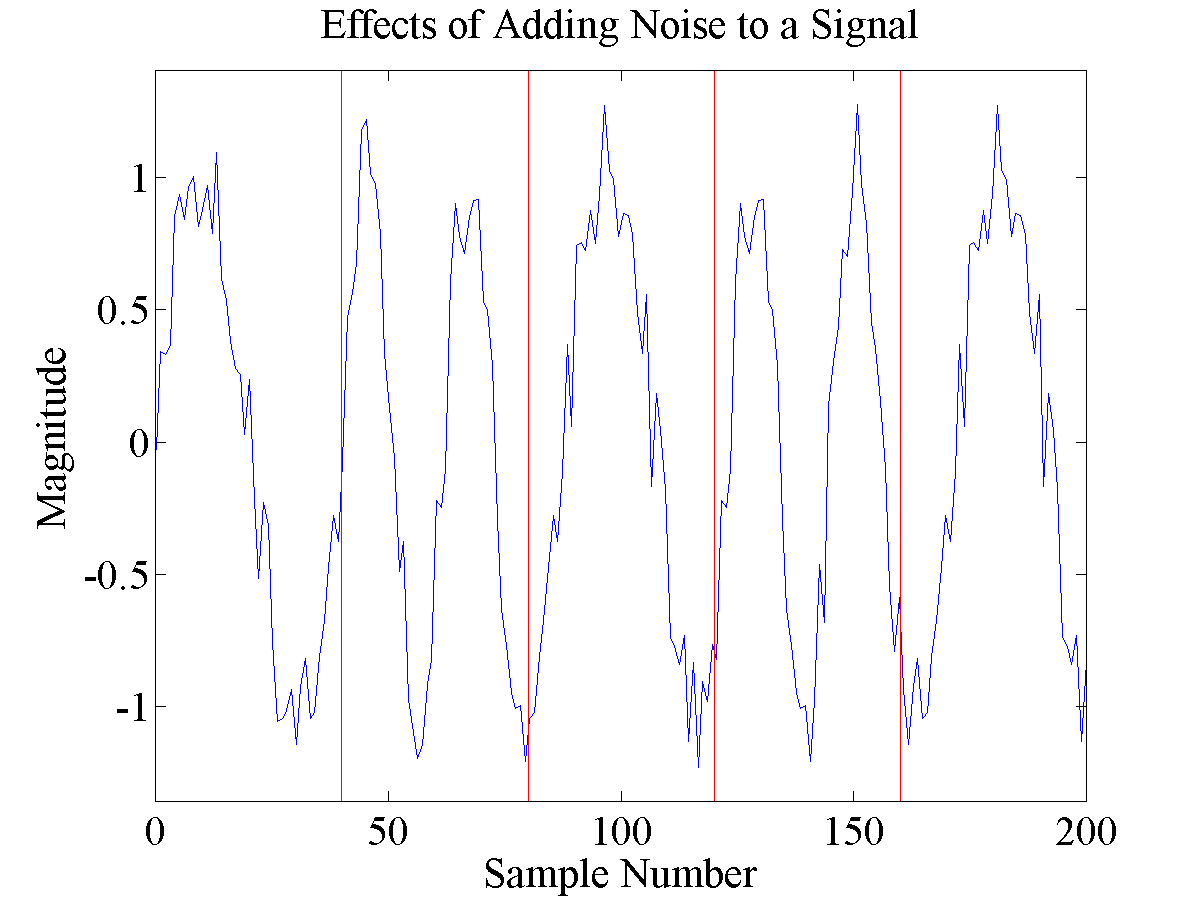
\includegraphics[width=0.75\linewidth]{images/EffectsofAddingNoisetoaSignal.png} 
	\caption{An example Bell 202 signal with white noise added.}
   \label{noiseExample}
\end{figure}

\section{Challenge: Emphasis}
Due to the fact that this is AFSK data being transmitted over a voice channel, emphasis becomes a concern. Preemphasis is when the the higher audio tones in a Frequency Modulated (FM) signal are intentionally increased and deemphasis is when that process is reversed on the receiving end to return the audio to a flat signal. Why emphasize the audio signal? This process of emphasis is not necessary, but the effects are desirable since it increases the signal to noise ratio in the RF signal by having the higher audio tones preemphasized \cite{Gibilisco1994}. The reason this is a concern is because the adoption of emphasizing and deemphasizing APRS signals is inconsistent. Some radios have data ports which bypass the emphasis step while other APRS users utilize the Mic and speaker ports of a radio which would utilize emphasis. This would mean that a signal transmitted out of a radio with a data port may not be emphasized, but then when received through the speaker out of another radio would be deemphasized. The effects of a non-emphasized signal being deemphasized can be seen in Figure \ref{emphasisExample}. This causes problems with the demodulation because it can not be assumed that the relative powers of each frequency will be equal since they will have different magnitudes in this case. 
\begin{figure}
  \centering
	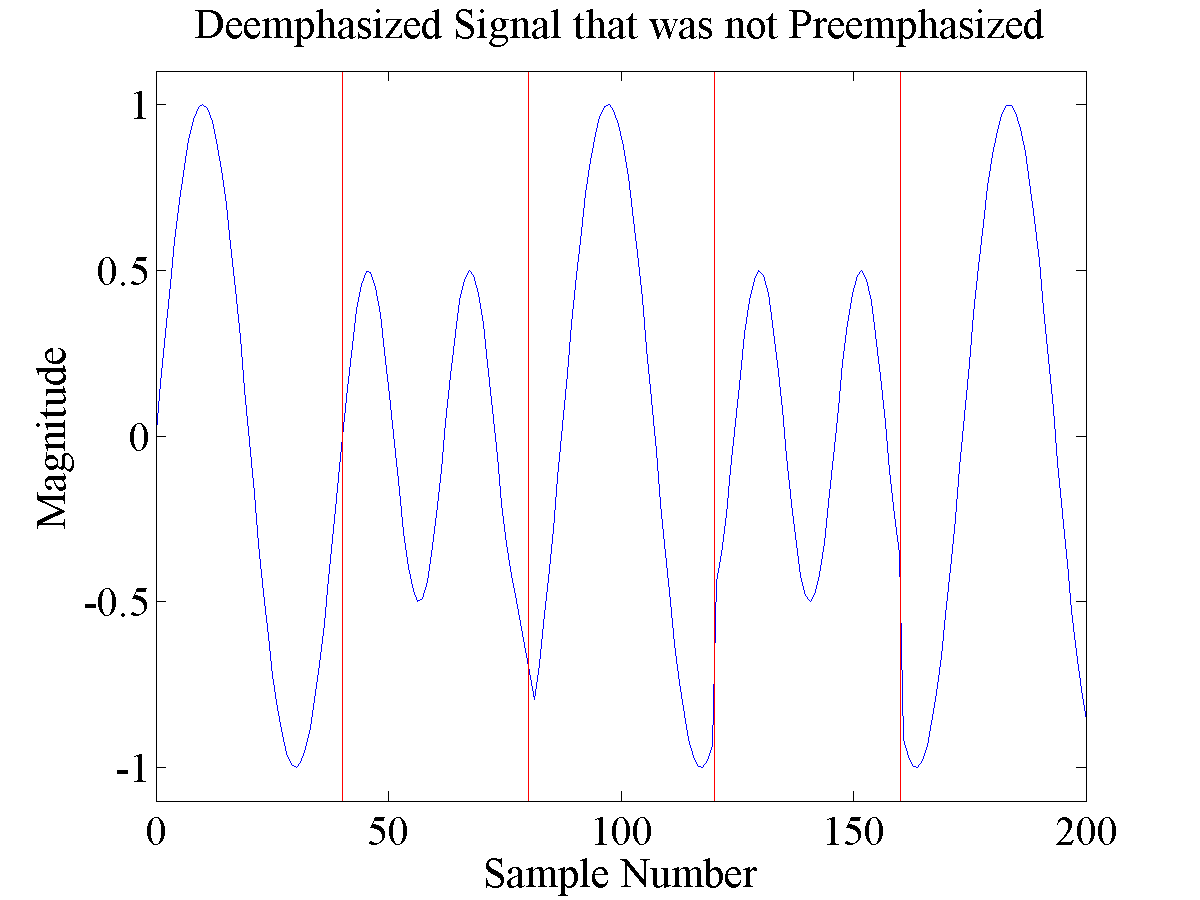
\includegraphics[width=0.75\linewidth]{images/DeemphasizedSignalthatwasnotPreemphasized.png} 
	\caption{An example signal that was not preemphasized, but was deemphasized.}
   \label{emphasisExample}
\end{figure}

\chapter{Demodulator Benchmarking}
In order to compare the results of the different demodulators a method of benchmarking must be instituted. Each one of the demodulators was tested using multiple audio files that have different characteristics. These different files as well as the advantage of using them in the benchmarking are explained in their corresponding section. It is worth noting that for each test audio file a sample rate of 48000Hz was standardized on since it works out nicely to 40 samples per bit period for 1200 baud digital communications. Although all the tests were performed with audio at a sample rate of 48000Hz, it is not expected that the results would change much if a different sample rate was chosen since items are calculated from file meta data as opposed to hard coded constants to suite 48000Hz audio.

\section{Plain, Straight, and Clean Packets}
These audio files were just what the title implies - straight packets. What is meant by straight packets is that they are pure "perfect" 1200Hz and 2200Hz tone audio samples. There is no noise introduced through artificial or natural means such as noise introduced through the intrinsics of using RF and the medium. Although these files do not provide meaningful results for hardware or already implemented software solutions (since these devices will be able to decode every packet in the audio file) it still provides a good starting point for getting new algorithms up and running. Two of these clean files were generated. One was generated from an OpenTracker creating packets with a counter and the text "The quick brown fox jumps over the lazy dog". This audio file contained a total of 40 packets and proved to be short enough to allow for quick cross checking as modifications were made. The second file was generated in software using Toledo's javAX25 package. All that is relevant at this point is that it has perfect levels (1200Hz and 2200Hz tones are at the exact same level) and contains 200 packets making the file quite a bit longer. An example segment from the 200 packet audio file can be seen in Figure \ref{gen200Segment}.
\begin{figure}
  \centering
	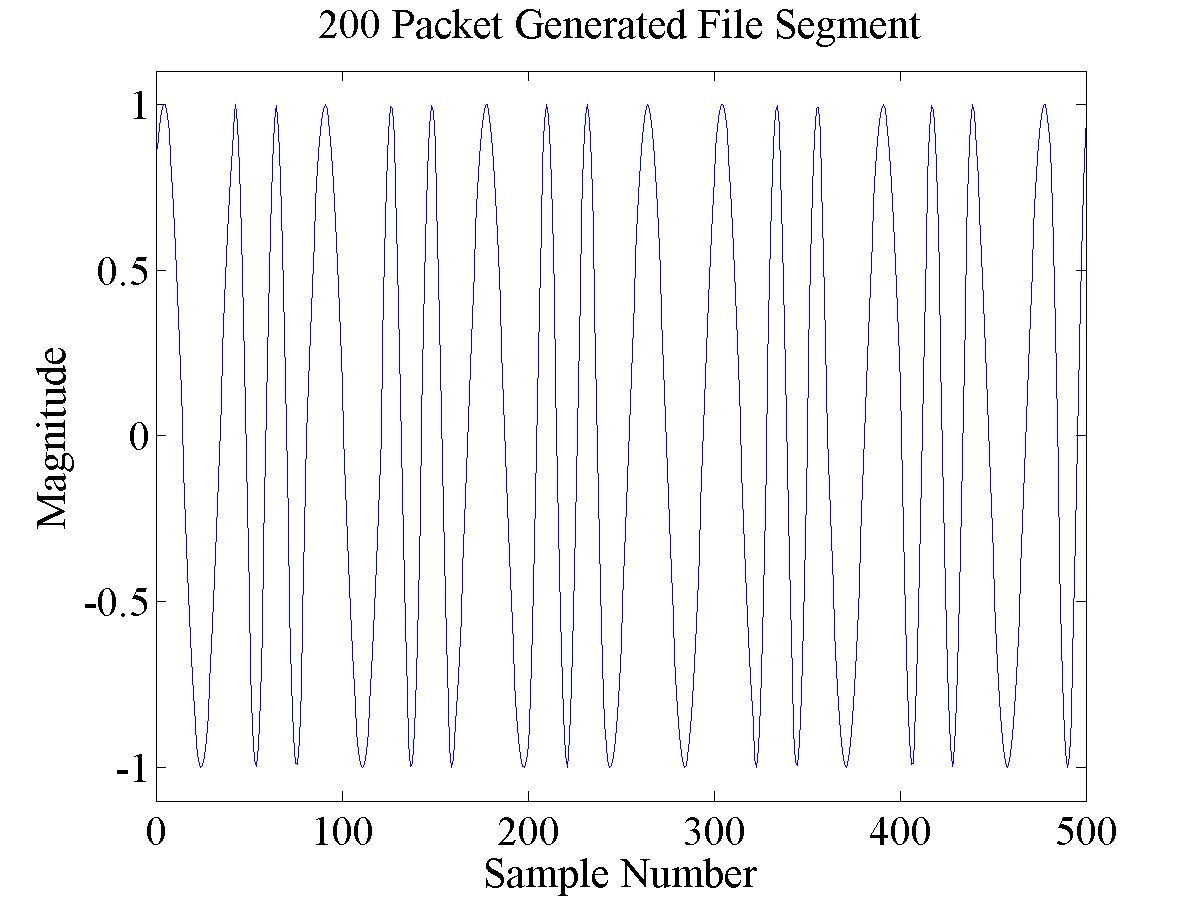
\includegraphics[width=0.75\linewidth]{images/200PacketGeneratedFileSegment.png} 
	\caption{Example of the AFSK present signal in the 200 packet generated file.}
   \label{gen200Segment}
\end{figure}

\section{White Noise Testing}
The second test file that was used on the demodulators was the 40 packet OpenTracker file mentioned in the previous section with added artificial white noise. An advantage of this file is that its contents are known while still being a reasonable benchmarking file. No demodulator could demodulate all the packets out of the file as the noise was increased all the way up to a signal to noise ration (SNR) of 0.5. There were total of 10 steps of increasing noise meaning that at each noise level there were approximately 4 packets. This noise was added to the original audio file using the audio editing program Audacity \cite{Mazzoni}. Although this file does not directly characterize what is introduced by RF, it provides a reasonable test simulating the effects of a decreased SNR on the audio signal. An example segment from this white noise added file can be seen in Figure \ref{OT3TestwNoiseSegment}.
\begin{figure}
  \centering
	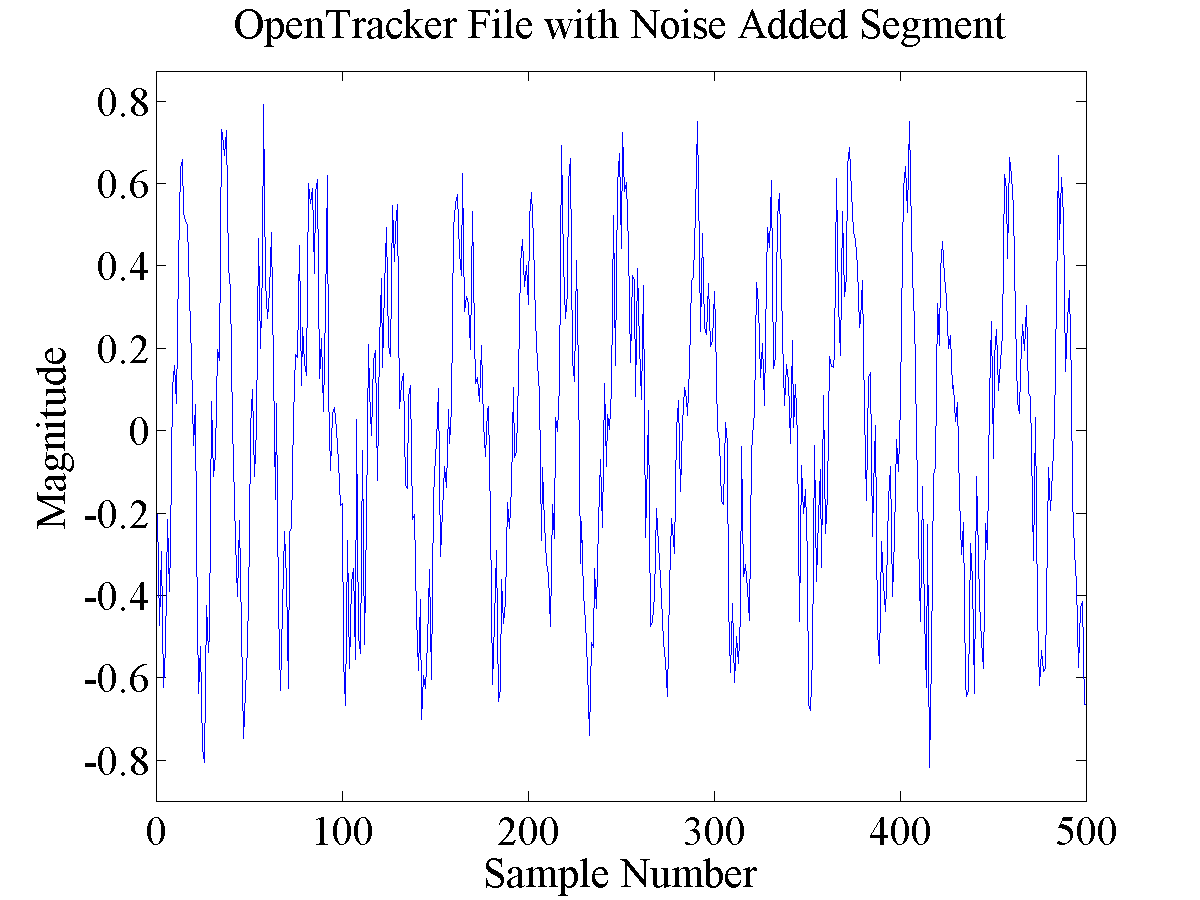
\includegraphics[width=0.75\linewidth]{images/OpenTrackerFilewithNoiseAddedSegment.png} 
	\caption{Example of a generated AFSK signal with artificial white noise added.}
   \label{OT3TestwNoiseSegment}
\end{figure}
 
\section{Los Angeles APRS Test Recordings}
%:04-25:45 57/min averaging over the first 3 minutes
This next benchmark is the de-facto benchmark for demodulators. The idea behind it is simple, yet it provides a very comprehensive test. The author of this file recorded on air APRS traffic in the Los Angeles Area for 45 minutes. He then removed segments of no traffic and condensed 45 minutes of live recording down to about 25 minutes \cite{Smith2009}. The nice thing is that it is real traffic which contains all of the real life situations including stations close to the receiver, far from the receiver, moving, stationary, different transmit power levels, different hardware, and varying content just to name a few. One disadvantage is that since it is just a random recording of traffic on the air, there is no definitive answer of how many packets are in the file. After listening to the audio file by ear it is approximated that there are a total of about 1463 packets by listening to the first 3 minutes as a sample and extrapolating to the length of the audio segment. This is considered \textit{the} file use for benchmarking in the community and when people discuss the performance of their demodulator, they quote it in how many packets they were able to successfully decode out of this file. An example segment from this off air recording of APRS traffic can be seen in Figure \ref{Track1Segment}. This is just one of the audio files on this author's test CD and is in fact the first one on the CD, so it will be referred to as Track 1. This was the the file that was most important to the testing, but the author also has a second version of this file in Track 2. The only difference between Track 1 and Track 2 is that an audio filter was used to create Track 2 which had the result of being a deemphasized version of Track 1. 
\begin{figure}
  \centering
	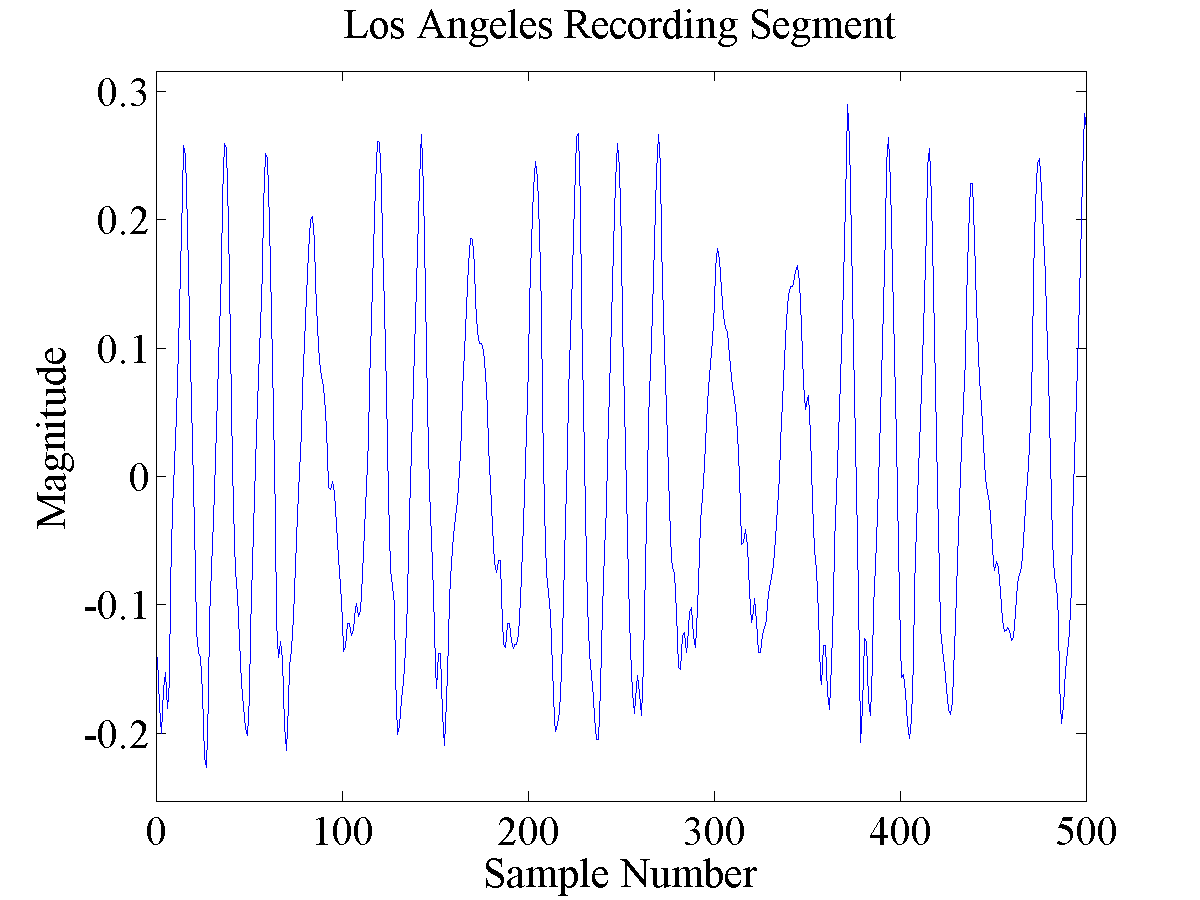
\includegraphics[width=0.75\linewidth]{images/LosAngelesRecordingSegment.png} 
	\caption{Example of the AFSK present signal in Track 1 of the Los Angeles Recording Test File.}
   \label{Track1Segment}
\end{figure}

\chapter{Testing}
In order to be able to evaluate the results from this research, each demodulation technique considered needs to be tested and the number of packets that each technique was able to successfully decode needs to be compared. From this analysis, it will be seen which techniques are effective and are able to decode relatively more packets as opposed to those that decode fewer. In order to validate the techniques results for dedicated hardware will also be collected for comparison. The testing for both the dedicated hardware and the software algorithms will be described in the corresponding sections below.

\section{Hardware Testing Setup}
The testing setup for the hardware is fairly simple since they are basically black boxes that just need to be supplied with the correct inputs. Each piece of hardware has two connections; one is the radio port, and the other is the serial connection. As the name implies, the radio port is used to be able to interface with the radio. This port has connections such as transmit audio, receive audio, push-to-talk (PTT), supply voltage (VCC), and ground. A digram of the common radio port can be see in Figure \ref{RadioPortPinout} and found in any manual including those of Argent Data\,\cite{Systems2013}. Since this was common between multiple pieces of hardware, a simple break-out board was created that allowed for a more universal audio transport mechanism of 3.5mm tip-ring-sleeve connectors, and also a 2.5mm barrel jack for power. This was much simpler than actually interfacing with a radio since the audio could just be played from a computer into the device; this device can be seen in Figure \ref{BreakOutBoard}. 

\begin{figure}
  \centering
	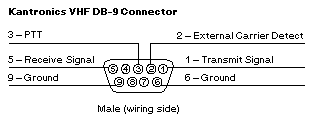
\includegraphics[width=0.75\linewidth]{images/RadioPortPinout.png} 
	\caption{Example Radio Port pin out for Kantronics, also consistent with others including OpenTrackers\,\cite{Martin2014}.}
   \label{RadioPortPinout}
\end{figure}
\begin{figure}
  \centering
	\includegraphics[width=0.75\linewidth]{images/BreakOutBoard.png} 
	\caption{Break-out board fabricated for hardware testing. There are two audio ports on the board; one for audio in and the other for audio out. On the right is the barrel jack fro supplying power.}
   \label{BreakOutBoard}
\end{figure}

\section{New javAX25 Demodulator Testing Framework}
Included within the javAX25 suite was a testing application that could both generate and decode packets. However, it was limited to only being able to specify one audio file and one demodulation algorithm. Using this test file as a basis, a new testing application was created that allowed for the multiple demodulators to be compared side by side against multiple audio files with a single run of the application. In addition to the output being printed to the console, the output was also saved to a file. Having these features in the testing application allowed for a much more streamlined analysis of all the algorithms collectively and tuning individual algorithms. One very convenient aspect of programmatically testing is that it is very easy to add a loop to try a range of tuning parameters and then look at the results to decide what is the best option. All of the results listed in the following chapter are from the testing application and mechanism described here.

\chapter{Implementation}

This chapter will go through all of the implementation details of each algorithm implemented. They will be presented in order of simplicity, with the more intricate ones presented last. This also will introduce them mostly chronologically since a naive approaches allowed for more insight to be gained into the JavaAX25 software package before implementing more complicated algorithms. In addition to giving a brief overview of each implementation some performance data will be provided, but all of the data will be presented in the Results Chapter. To see detailed 

\section{Strict Zero Crossing Demodulator}
This approach used the technique of finding zero crossings and then using those to determine the period. From the period the frequency was then calculated. For 1200Hz and 2200Hz tones zero crossings are expected every 833�s and 455�s respectively. If it was above 1700Hz it was assumed that a mark was present in the signal and if lower than 1700Hz a space must be present. The zero crossing were found by determined if the signal was negative and changed to positive or if it was positive and changed to negative. Although this algorithm was only able to decode a little over half of the packets as some of the other algorithms, it proved to be an important stepping stone into javAX25 and allowed for preparation into restructuring the project for added modularity of the filtering. With the first implementation Toledo's bandpass filters were not used and instead the previous three samples were averaged as a method of filtering to remove sample to sample noise.

\section{Zero Crossing Demodulator}
Building on the strict zero crossing this zero crossing demodulator tried to use some more intelligence in finding the zero crossings through additional processing. One reason that the strict zero crossing approach was thought to have relatively poor results was due to the previously introduced challenge of DC offset. If the signal doesn't actually cross zero then it will be very hard to find the zero crossings. This method keeps a window of history, it was arbitrarily chosen to be one bit period, and from this collection of samples the average is taken to use this as the baseline - or zero value. Instead of checking to see if the signal crosses zero, the signal is analyzed for going from either above to below or below to above this average value. This ended up having worse results than the strict zero crossing demodulator. This was due in part to the fact that 2200Hz signals even when properly centered around zero will not have an average of zero since it does not complete two fill periods within on bit period, tainting the average.

\section{Windowed Zero Crossing Demodulator}
With now having a good handle on utilizing zero crossing a new approach was taken to keeping history. Instead of using the history to calculate where "zero" is, what if how many zero crossings are within one period are observed. If a windows slightly shorter than one bit period is selected, then if there are only two crossings within that window it will correspond to a 1200Hz symbol being present. More crossings than two means that a 2200Hz symbols must be present. The thought behind taking this approach is that it would give some additional resiliency to noise by finding the average during that bit period through utilizing multiple zero crossing instead of individually analyzing every zero crossing. 

\section{Peak Detection Demodulator}
After making a simple zero crossing overly complicated, it was decided that maybe a different approach should be taken, specifically to look at a different part of the signal. It was considered that perhaps better performance could be achieved by looking at the peaks in the signal instead of the noisy zero crossing around ground, or not around ground if there are DC offset problems. The nice thing about this is that the difference between two consecutive peaks will be equal to the period of the underlying signal. Although the methodology is the same as the zero crossing for converting the period to the actual frequency it was perceived that this would give better results. It turns out that this method did not work as well as hoped due to the fact that local peaks were commonly discovered from the noise instead of the actual peak in the transmitted signal.

\section{Derivative Zero Crossing Demodulator}
After a failure with the peak detection demodulator a new approach was taken to finding "peaks." Instead of actually looking for the peaks, the zero crossing demodulator was revisited with a new spin. Instead of using the raw samples for determining the frequency using zero crossings, the derivative was to be used. The derivative was calculated by doing the same averaging as in the strict zero crossing approach and then subtracting the current average from the average two samples ago. It was thought that this would solve the DC offset problem for sure, but it turns out that this was not the larger problem. The problem was with using the zero crossing approach and this derivative implementation ended up just having very similar results to the strict zero crossing.

\section{Goertzel Filter Demodulator}
Finally moving away from approaches utilizing zero crossing methodologies, an approach using a Goertzel filters was implemented. The implementation was very simple and corresponds with that outlined in the Demodulation Techniques Chapter. Since it has to be applied onto a set of data, originally a window size was selected that was equal to one bit period so as to make sure that the data being processed was only that of one frequency, but after analyzing the effect of the window size on performance, a window size of slightly bigger than a bit period ended up being better. The optimal size was tested to be 135 percent of a bit period, and the reason why this worked better is because it gave more signal in the window for the filter to lock onto and essentially the window was only extended 18 percent on each side of a bit period. This over extension of the window is what led to being able to exceed the performance of the original correlator on unfiltered data.

\section{Phase Locked Loop Demodulator}
Next, the PLL demodulator was implemented. Using Lutus's python based software PLL initial testing was performed to see how it would work for tracking AX.25 signals \cite{Lutus2011}. Once the parameters were tuned sufficiently that it seemed to be staying locked onto the signal it was ported over to java and actually run as a demodulator. Once inside of the javAX25 framework additional tuning was done programatically instead of manually to further fine tune the performance. The final results were that it was not the winner, but comperable to the other top contenders, correlation and Goertzel filter.

\section{Mixed Preclocking Demodulator}
Finally with numerous simple algorithms implemented, or at least they may appear that way due to their relatively few lines of code, it was time to try something much more complicated. Something that would only be possible in software to see if it would shine. This approach and name preclocking comes from an abbreviation for predetermined clocking where packets are analyzed a whole packet at a time. The start and end are found and then the clocking and hence bit boundaries are predetermined before the actual demodulation takes place on a bit by bit basis as opposed to a sample by sample basis. Each one of the preceeding algorithms was on a sample by sample basis, meaning they had to make their best determination of bits elapsed using a little bit of history.

There are five different steps to the demodulation in the Mixed Preclocking Demodulator. First, flags are found in the signal so that the demodulation can happen one packet at a time instead of just blindly trudging forward through the packet sample by sample. Second, the derivative of the whole packet is taken to  determine the zero crossings. Third, frequency transitions are extrapolated from the derivative data. Fourth, the frequency transitions found in the packet are used to determine the clocking or bit boundaries. Finally, fifth the tone demodulation is done on a baud by baud basis. It was speculated that processing one packet at a time with the correct clocking to demodulate bit by bit would allow for very accurate demodulation.

Although, it was hoped that the results would be better, there were so many different methodologies being used that it was very difficult to tune. For instance the flags were found using the correlation approach, and the transitions using a derivative, and the final demodulation using the zero crossings. What were thought to be the advantages ended up being the challenges, but as predicted it did pretty well to still be considered one of the successful implementations. The intricate nature of this demodulator made it delicate which was noticed during the testing through the fact that it would not decode any packets unless a bandpass filter was used on the incoming data.

\section{Goertzel Preclocking Demodulator}
After the first attempt as a preclocking approach, it was thought that perhaps only using one methodology to perform all the different steps of demodulation would be at the very least simpler, and hopefully better. The perception that it might be better came from the fact that there was only one item to tune, the Goertzel Filter. Instead of having to worry about noise affecting zero crossings and the derivative potentially adding emphasis problems, only the filter has to be considered. Unfortunately the number of packets that this method decoded was not as many as the first Goertzel approach, or the previous preclocking. This was due to the fact that even though there was one underlying algorithm it was used in three separate instances, and each wanted slightly different tuning. The three instances were for flag detection, frequency transition detection, and the the final bit by bit demodulation.

\section{Goertzel Exhaustive Precklocking Demodulator}
The final algorithm implemented was just a manner of verification, and another one that could only be performed in software. Instead of analyzing packets one at a time using flags as the start and end points, a whole array of data that had a length equal to the number of samples that a packet if the maximum length would have. Every time a few more samples came in, every single clocking was attempted on the large array of data just to see what packets could be decoded by exhaustively searching for data. The performance of this algorithm in terms of time to run was much longer. For instance the mixed preclocking and original Goertzel preclocking took 3 minutes and 5 seconds and 2:36 to run respectively while this exhaustive search took 26:48 on the 25 minute 49 second Track 1 of the test suite. This means that a 2.1Ghz Intel i7 (i7-3612QM) could not process the audio file in less time than elapses during the content of the audio file. With this being the case, that means that with live data this approach would not work since it would continuously fall behind. Gratefully, this approach only decoded an additional 15 packets that the Correlation, original Goertzel (non-preclocking), and PLL did not decode. This result could be used to make the argument that the few more packets decoded is not worth the vast number more CPU cycles it take to achieve it.


\chapter{Results}
This results chapter is meant as a mechanism to present all of the data that was collected on the performance of different demodulators. All of the demodulators that were tested in the course of this research will be shown, whether it be dedicated hardware or software. The first results that will be shown are those of the dedicated hardware, being TNCs and Argent Data's OpenTrackers. Following the hardware will be the software implementations. Following these two categories will be some general comparisons between them.

\section{Dedicated Hardware Results}
In the scope of this research a total of 12 pieces of hardware were tested. They include Argent Data's OpenTracker 2, OpenTracker 3, OpenTracker USB, OpenTracker 3 Micro, Kantronics Kam, two Kantronics Kam Plus, two AEA PK-88, a PK-232, a PK-232MBX, and an MFJ-1278. Hardware models for which more than one was tested will be differentiated by a number in parentheses following the model number. Please note that on the figures OpenTracker will be abbreviated OT.

The first two tests consisting of clean packets - 40 generated from the OpenTracker and 200 using Toledo's suite - was relatively uninteresting. Essentially every piece of hardware decoded all 40 and all 200 packets. The only anomalies to this were that the OpenTracker USB was only able to decode 39 and 193 out of the 40 and 200 packet files respectively. Additionally the OpenTracker 3 Micro missed one packet in the 200 packet file to only decode 199. Since there is no real way to debug and see the cause of decoding relatively fewer or more packets just the data for these hardware items is presented as it was measured to allow for comparison to the software. This will continue to be the case for the remainder of this hardware section.

Following the two easy files the next file is same content as the file with 40 packets in it, with the only difference being that noise was progressively added. In Figure \ref{allHardwareOT3Noise}, the two PK-88s stand out for being able to decode 25 of the 40 packets in this file.

 \begin{figure}
  \centering
	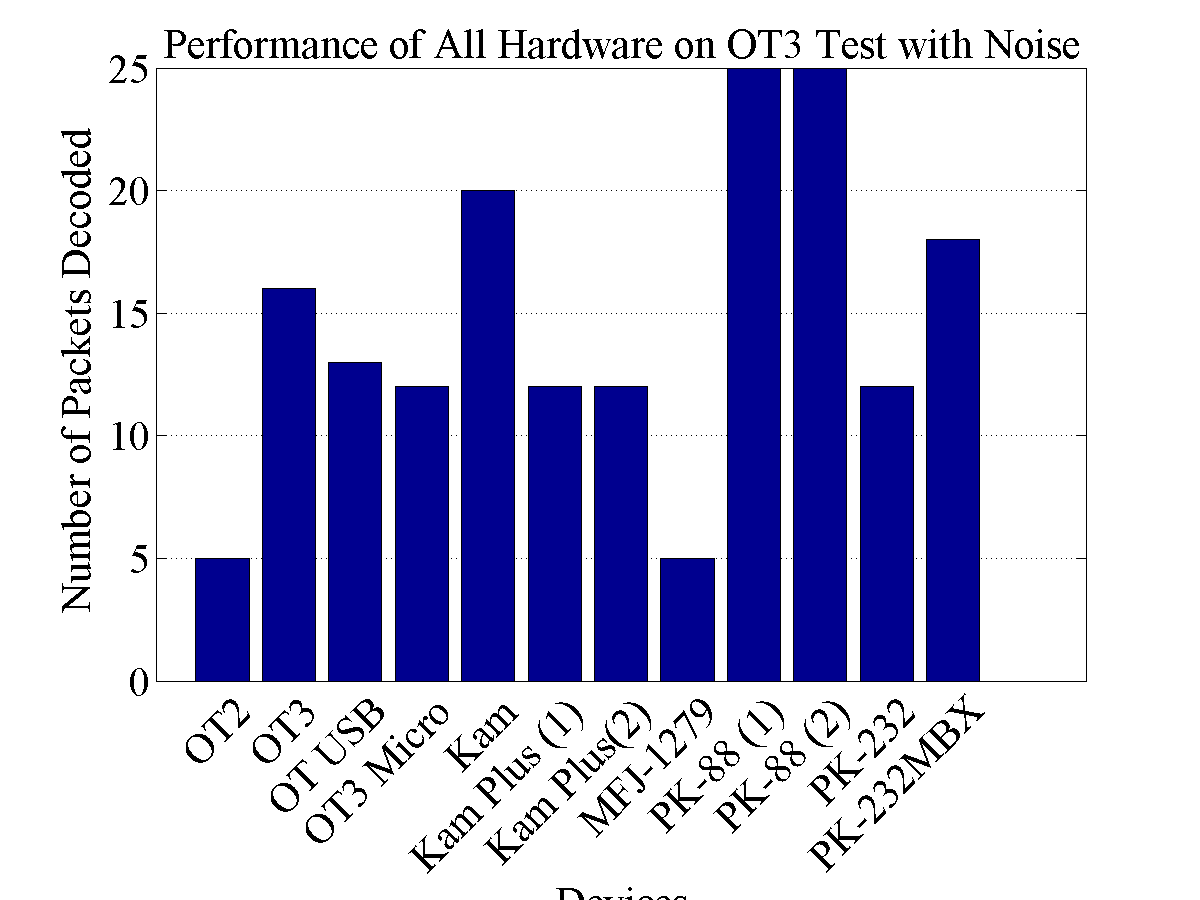
\includegraphics[width=0.75\linewidth]{images/PerformanceofAllHardwareonOT3TestwithNoise.png} 
	\caption{Number of packets successfully decoded for all tested hardware on the OpenTracker 3 test file with noise.}
   \label{allHardwareOT3Noise}
\end{figure}

The next two files are the ones that were used most extensively in the testing for comparison and tuning. Primarily the first, which is just a recording of traffic off the air. They are Track 1 and 2 from the APRS CD mentioned in the Demodulator Benchmarking Chapter. The results from Track 1 are in Figure \ref{allHardwareTrack1} and Track 2 in Figure \ref{allHardwareTrack2}. The top three performances of the hardware on Track 1 were the PK-88 (2) with 1007 packets decoded, the Kam with 988 Packets, and the Kam Plus (2) with 985 Packets. For Track 2 the top hardware was the Kam Plus (2) with 998, the Kam Plus (1) with 967, and the Kam with 938.

 \begin{figure}
  \centering
	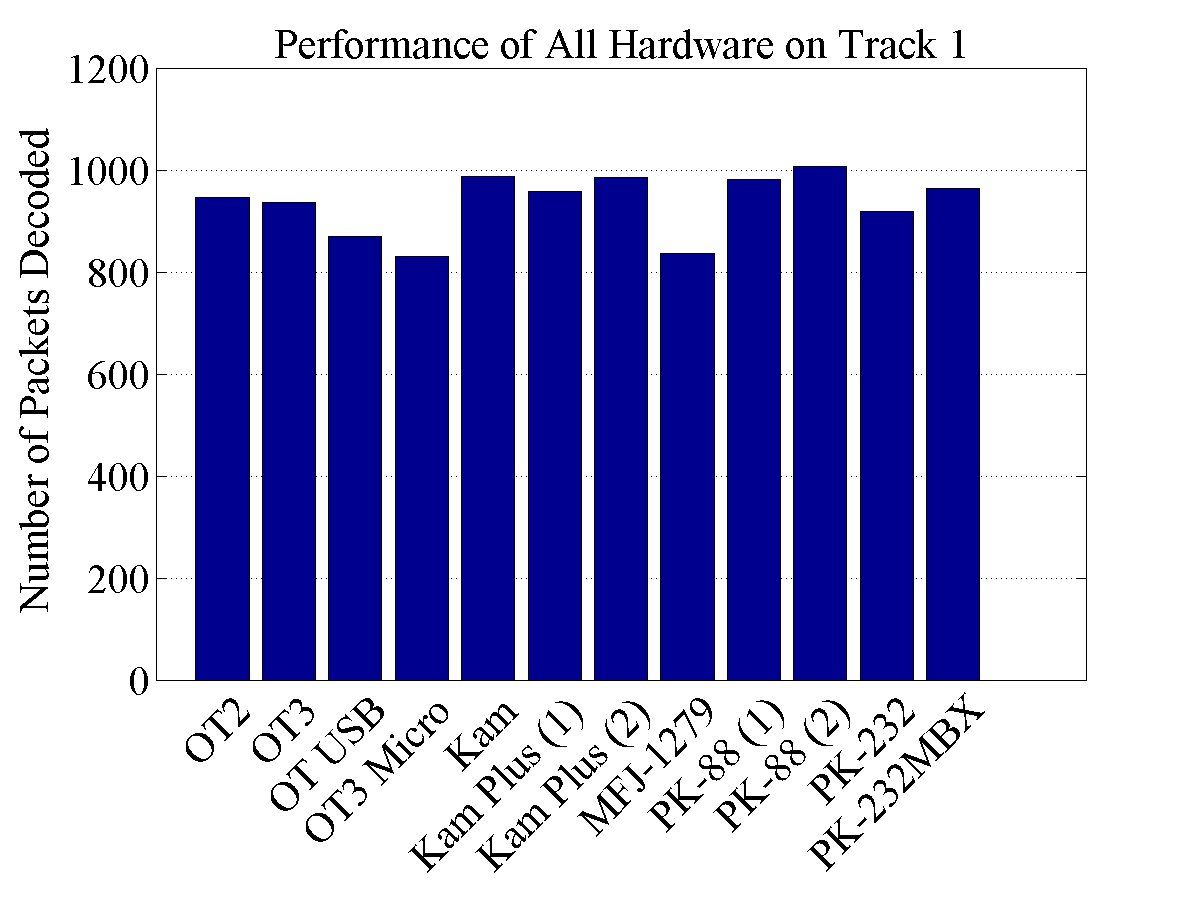
\includegraphics[width=0.75\linewidth]{images/PerformanceofAllHardwareonTrack1.png} 
	\caption{Number of packets successfully decoded for all tested hardware on the Track 1 test file.}
   \label{allHardwareTrack1}
\end{figure}

 \begin{figure}
  \centering
	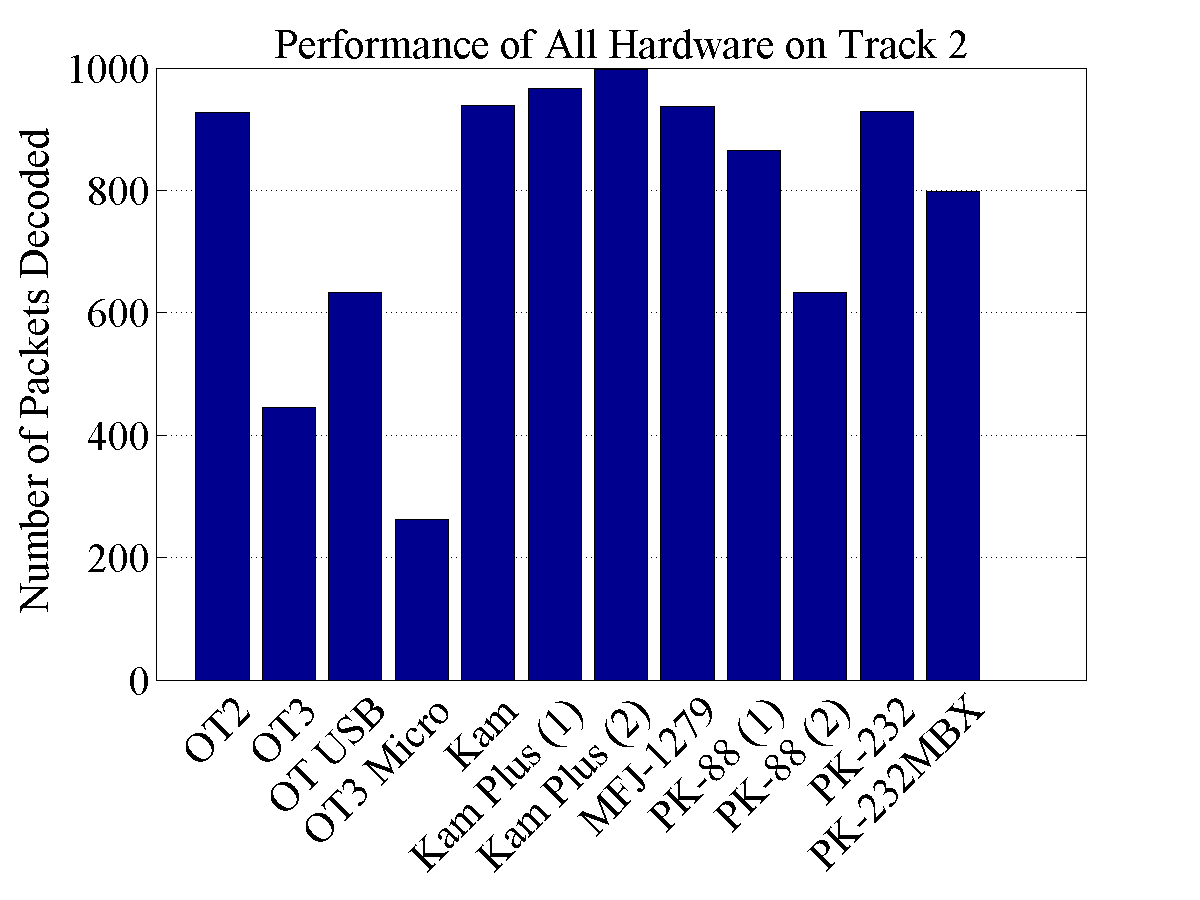
\includegraphics[width=0.75\linewidth]{images/PerformanceofAllHardwareonTrack2.png} 
	\caption{Number of packets successfully decoded for all tested hardware on the Track 2 test file.}
   \label{allHardwareTrack2}
\end{figure}

Using these results the best numbers for the hardware were 40 packets decoded from the Open Track 3 test, 200 from the javAX25 generated file, 25 from the Open Tracer 3 test with added noise, 1007 from Track 1 of the LA test suite, and 998 from Track 2. These best results can be used as a comparison for the software.

\section{Software Results}
In this section the number of packets that each of the demodulators in the javAX25 package was able to decode will be presented, highlighting those that were newly implemented in the course of this research. This will include the correlation approach that was already implemented before the start of this research as well as all of the new algorithms that were outlined in the previous chapter on Implementation. However, before getting the results from javAX25 there is one more data set to be introduced which is the results from another software based demodulation from AGW Packet Engine. Using this software 40 packets were decoded from the OpenTracker 3 test, 200 from the javAX25 generated file, 21 from the OpenTracker 3 test with added noise, 967 from Track 1 of the LA test suite, and 497 from Track 2. The results from javAX25 end up being on par with these results as well as those of the hardware.

With a total of 13 algorithms implemented, some did well and others not at all, so as in the section on hardware results, all of the data will be presented followed by a focus on those that performed the best. In the new javAX25 software implementation the filtering was moved from its original location of being on a per demodulator level basis to a central location that allowed each of the algorithms to utilize it. Some of the algorithms ended up relying on it after tuning and others could remain independent. As such, in order to present all of the data each algorithm will not only have a result for each of the 5 test files, but also for each of the three filters used on the data. The three filters used are no filter, a 900-2500Hz bandpass filter, and the same bandpass with a 6dB attenuation of 1200Hz tones to combat the signals that were not emphasized when transmitted but were deemphasized when received. For instance, for the Zero Crossing demodulator there will be three values for the OpenTracker 3 Test file, one at each filtering, and so on for the remaining 4 test files.

In terms of the data, correlation data will be on the far left of all the plots which was the current algorithm that it was the goal to beat. The performance of no filter on the OpenTracker 3 Test can be seen in Figure \ref{OT3FiltNo}, Figure \ref{OT3Filt0} shows data with the bandpass filter, and the emphasizing filter results in Figure \ref{OT3Filt6}. It can be observed that zero crossing did not favor the filters, others were resilient, and preclocking thrived. The Generated 200 Test file is the only file that the peak demodulator performed comperably to the other techniques on. The unfiltered data from this test is in Figure \ref{Gen200FiltNo}, the bandpass data in Figure \ref{Gen200Filt0}, and the results of emphasizing the signal in Figure \ref{Gen200Filt6}. Although the generated 200 packet file and the OpenTracker test file had similar results, the results for the generated 200 were better. This can be attributed to the fact that this file has only ever existed in the digital realm, it was made and consumed there, as opposed to existing in the physical world and then recording it.

\begin{figure}
  \centering
	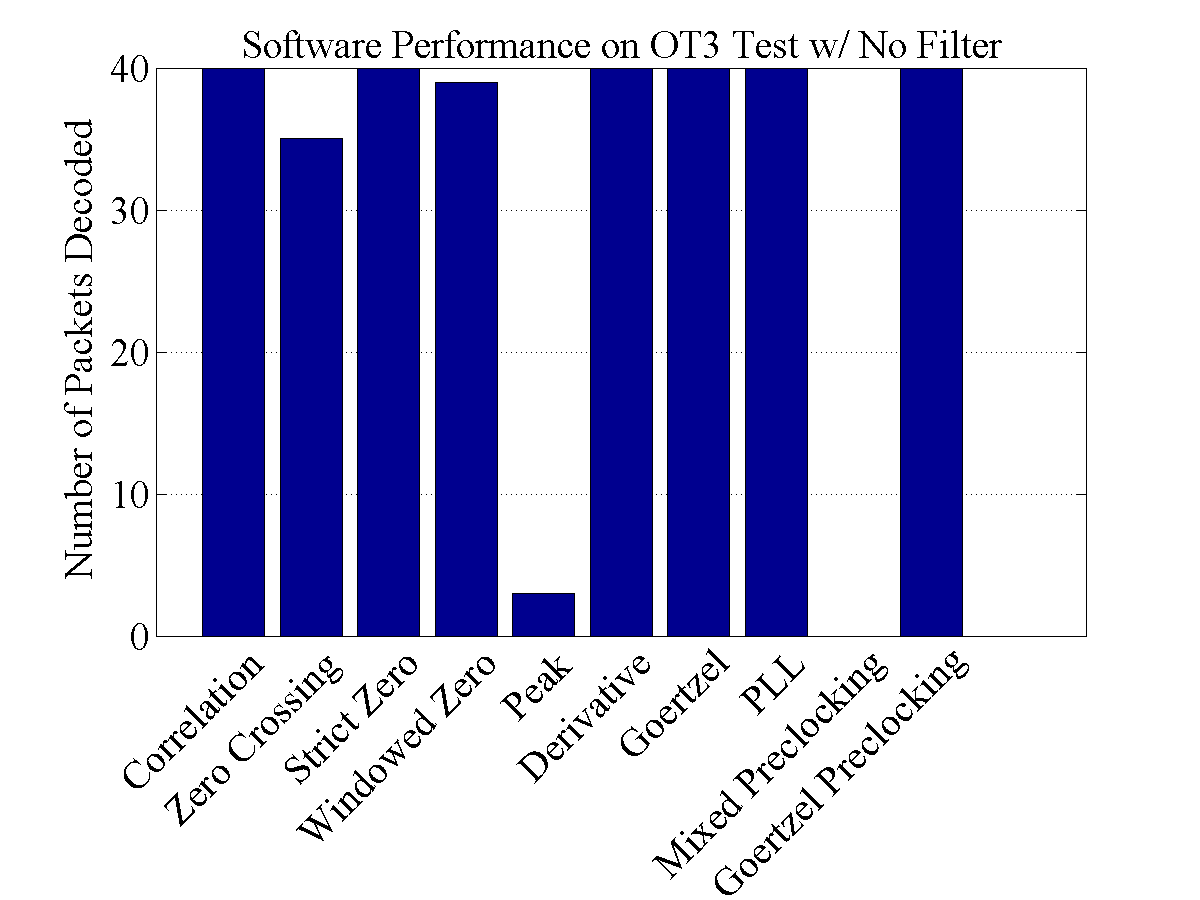
\includegraphics[width=0.75\linewidth]{images/SoftwarePerformanceonOT3TestwNoFilter.png} 
	\caption{Performance of software on the raw signal from OpenTracker 3 Test.}
   \label{OT3FiltNo}
\end{figure}
\begin{figure}
  \centering
	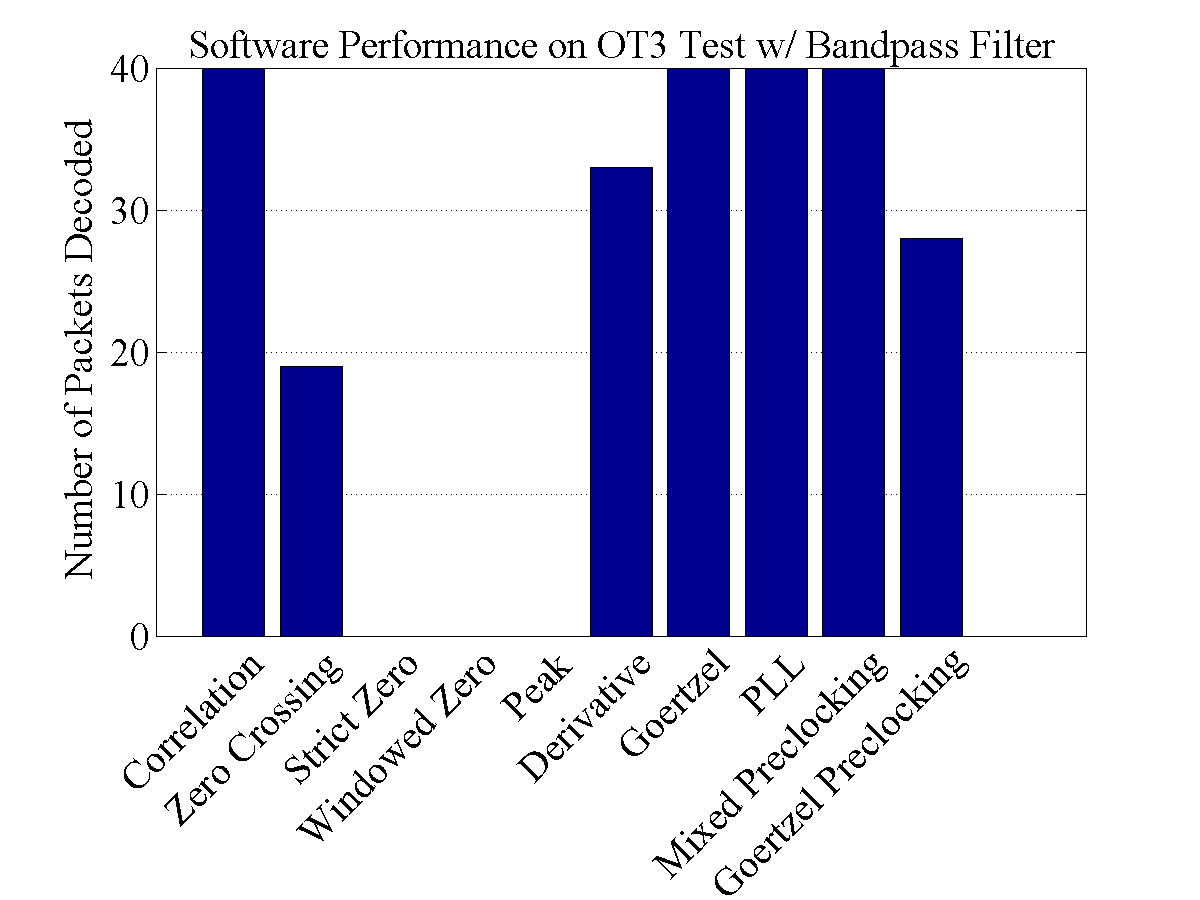
\includegraphics[width=0.75\linewidth]{images/SoftwarePerformanceonOT3TestwBandpassFilter.png} 
	\caption{Performance of software on OpenTracker 3 Test with a bandpass filter.}
   \label{OT3Filt0}
\end{figure}
\begin{figure}
  \centering
	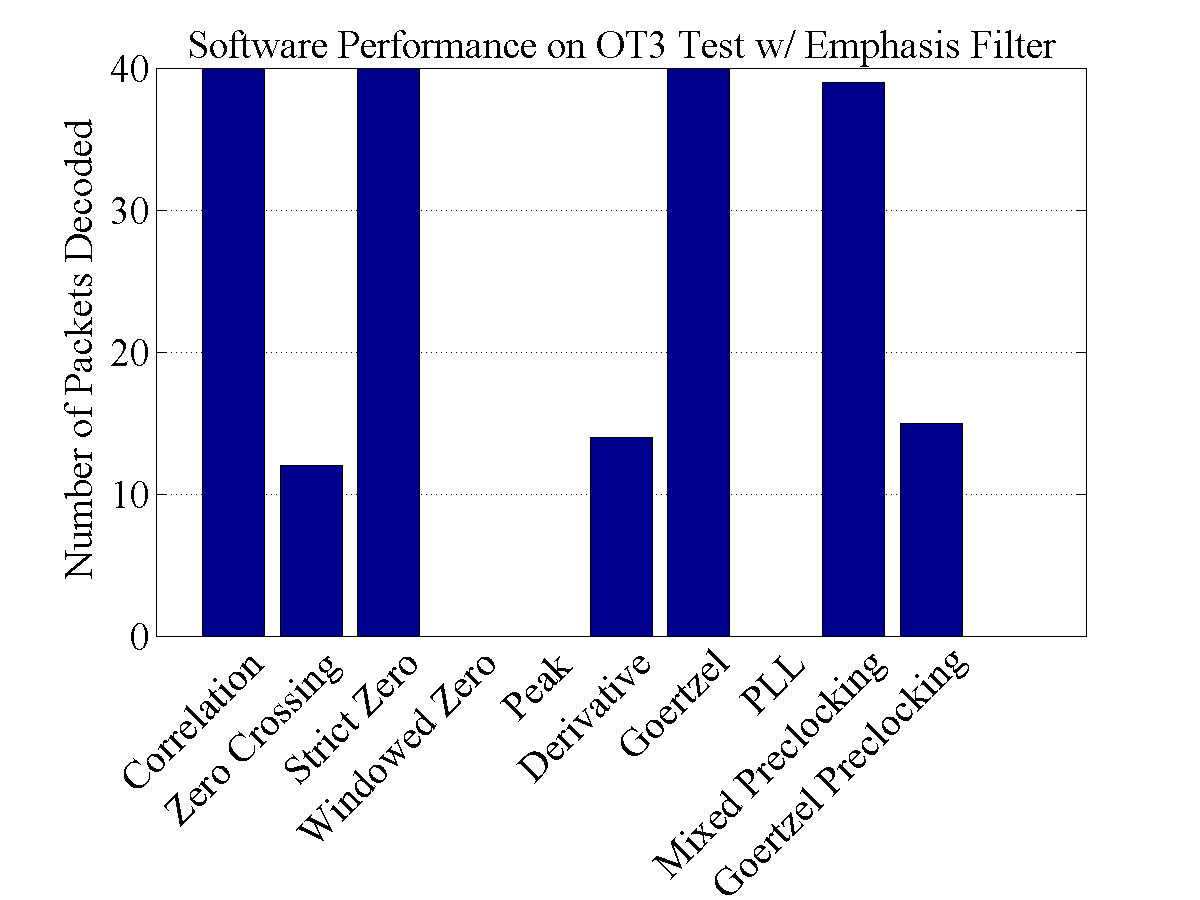
\includegraphics[width=0.75\linewidth]{images/SoftwarePerformanceonOT3TestwEmphasisFilter.png} 
	\caption{Performance of software on OpenTracker 3 Test with an emphasis filter.}
   \label{OT3Filt6}
\end{figure}
\begin{figure}
  \centering
	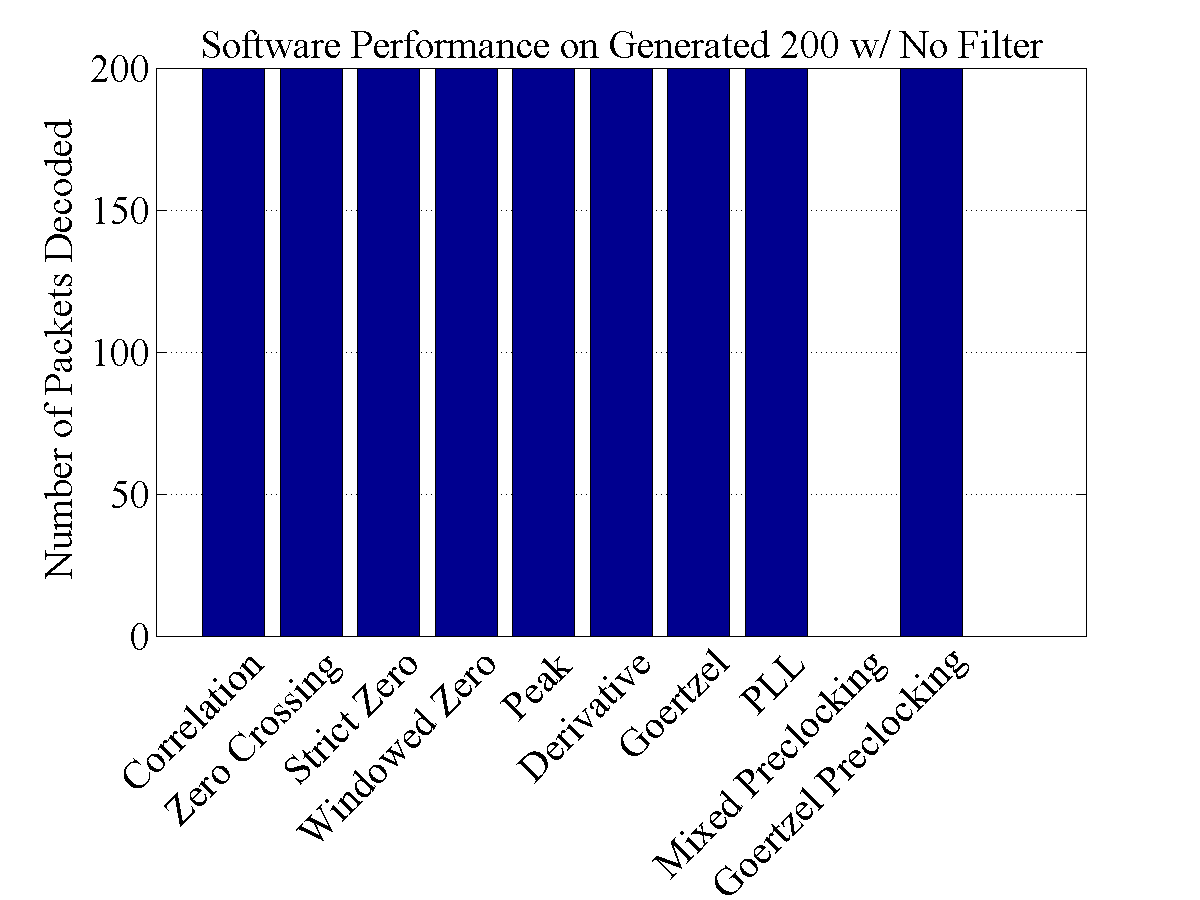
\includegraphics[width=0.75\linewidth]{images/SoftwarePerformanceonGenerated200wNoFilter.png} 
	\caption{Performance of Software on the raw signal from Generated 200.}
   \label{Gen200FiltNo}
\end{figure}
\begin{figure}
  \centering
	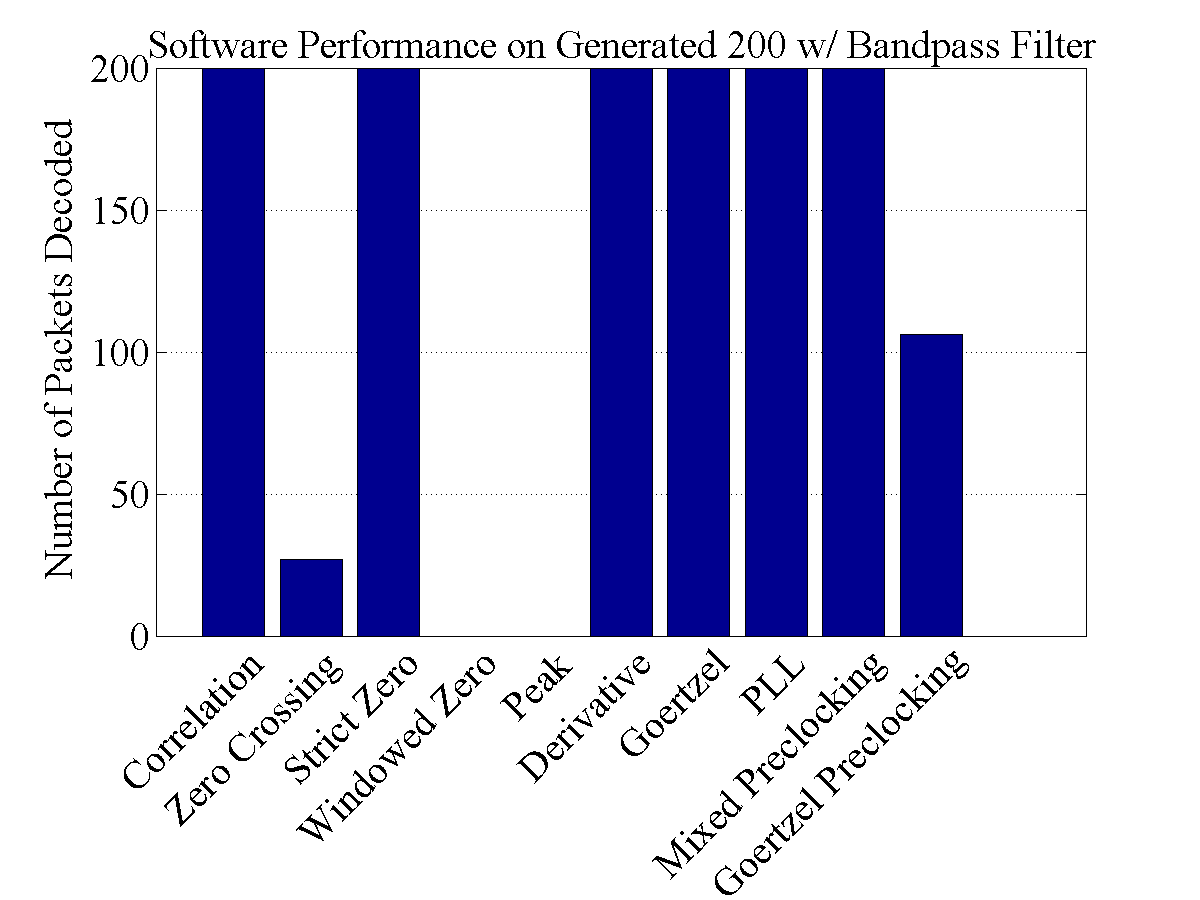
\includegraphics[width=0.75\linewidth]{images/SoftwarePerformanceonGenerated200wBandpassFilter.png} 
	\caption{Performance of software on Generated 200 with a bandpass filter.}
   \label{Gen200Filt0}
\end{figure}
\begin{figure}
  \centering
	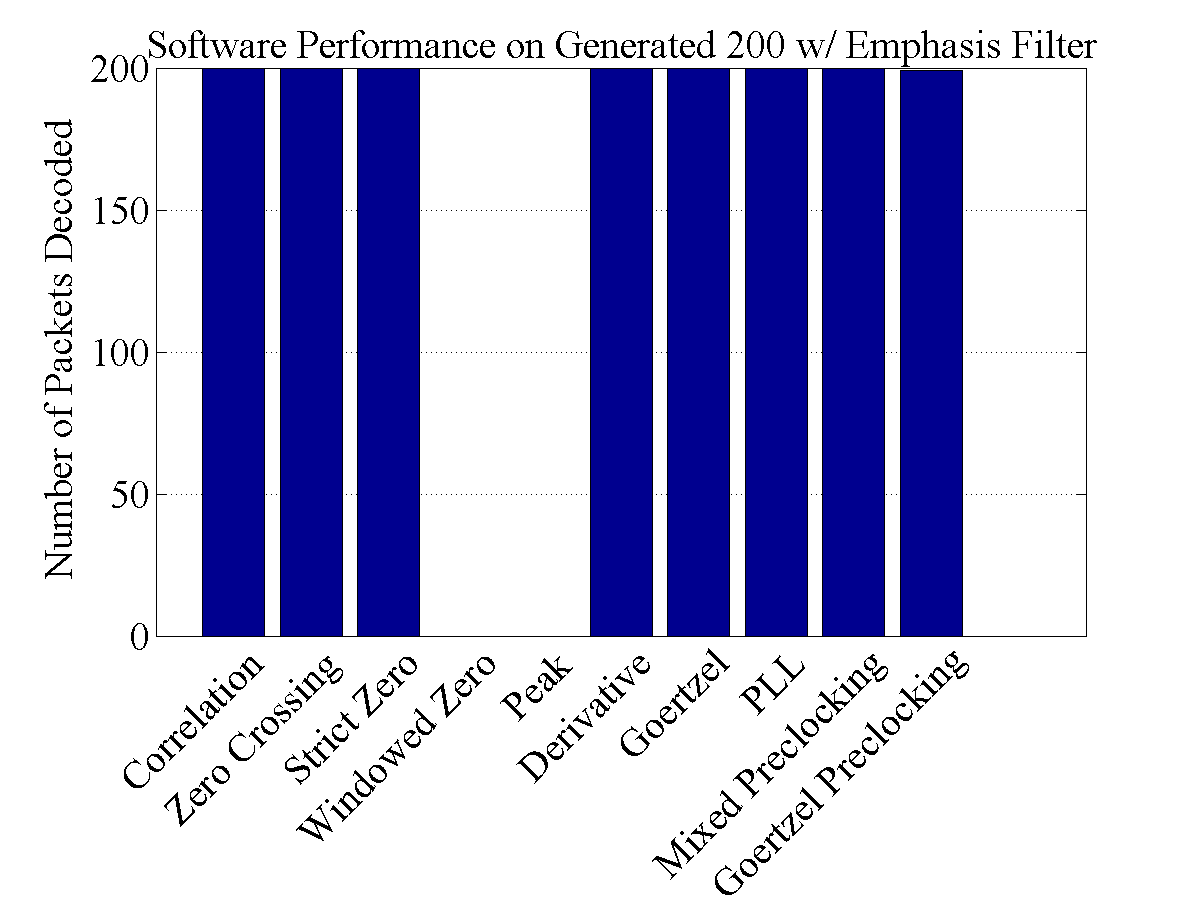
\includegraphics[width=0.75\linewidth]{images/SoftwarePerformanceonGenerated200wEmphasisFilter.png} 
	\caption{Performance of Software on Generated 200 with an emphasis filter.}
   \label{Gen200Filt6}
\end{figure}

Again, moving on from the "easy" files the performance of the software demodulators on the OpenTracker 3 Test with the noise added can be seen. Figure \ref{OTNoiseFiltNo} shows the data for the unfiltered file, Figure \ref{OTNoiseFilt0} shows bandpass filter data, and Figure \ref{OTNoiseFilt6} shows data from the emphasis filter. Two algorithms really start to shine as being comparable, and in some cases better, than the correlation demodulator. Those are the Goertzel Filter Demodulator and the PLL Demodulator. Although this is not data that was actually transmitted or received, these two start so who promise. Even the Strict Zero crossing can be seen doing well once the audio file is emphasized, but it doesn't stand up to the competition in the next two test files.

\begin{figure}
  \centering
	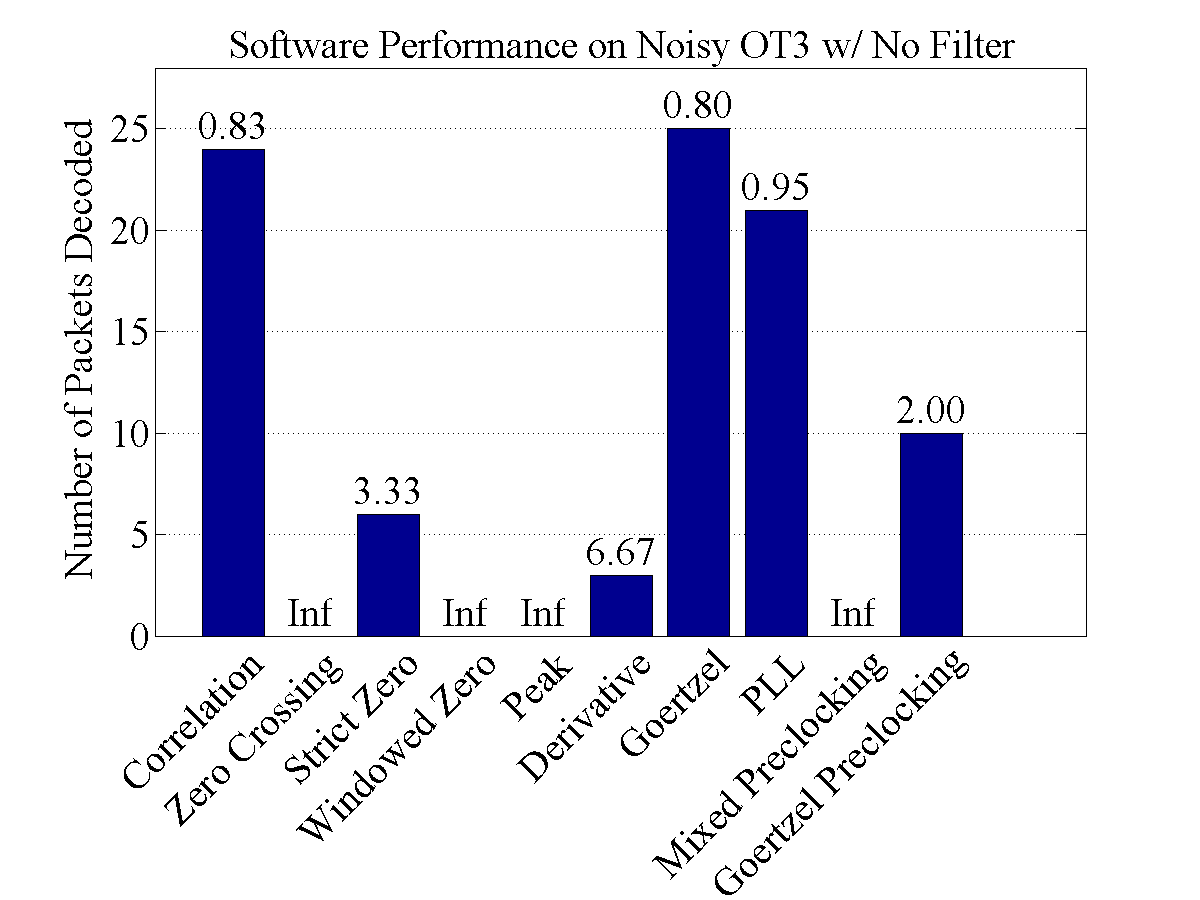
\includegraphics[width=0.75\linewidth]{images/SoftwarePerformanceonNoisyOT3wNoFilter.png} 
	\caption{Performance of software on the raw signal from OpenTracker Test with noise added.}
   \label{OTNoiseFiltNo}
\end{figure}
\begin{figure}
  \centering
	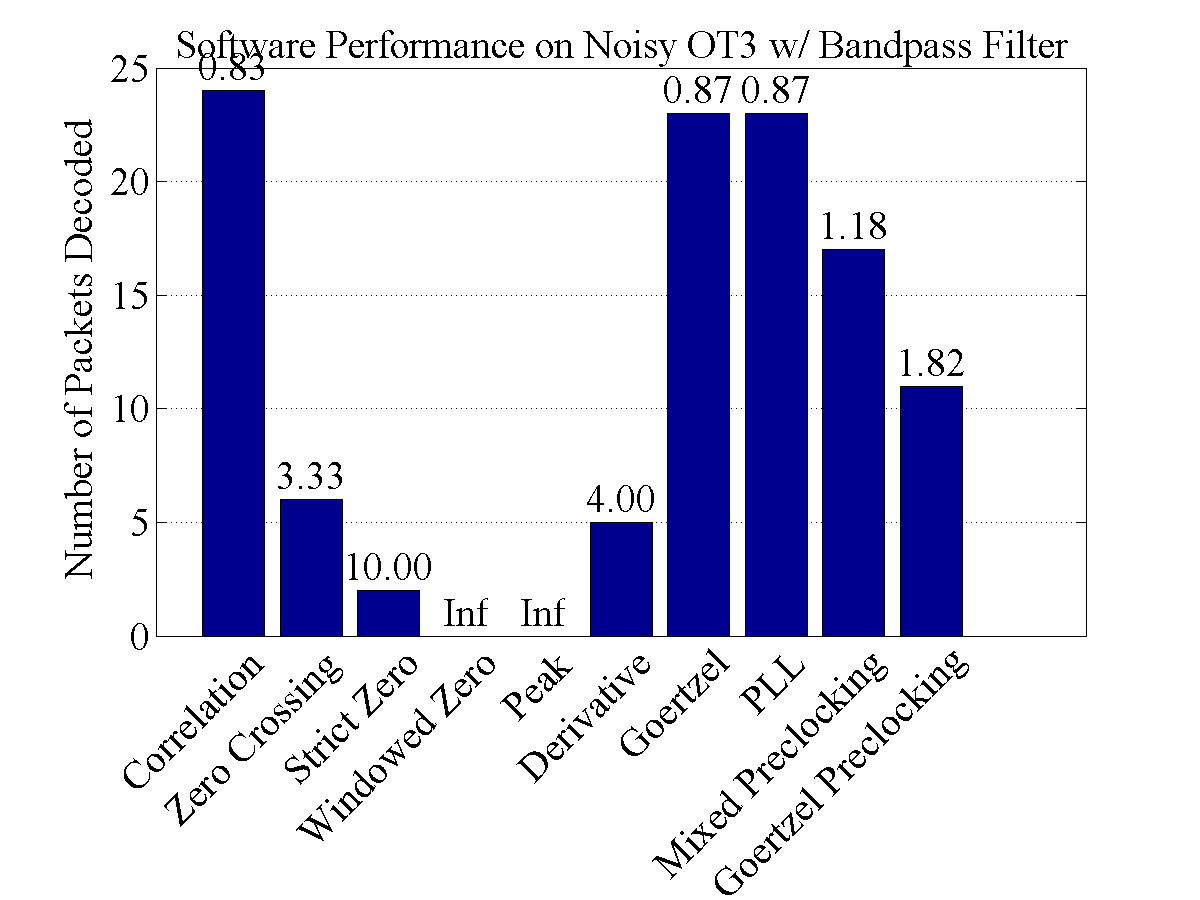
\includegraphics[width=0.75\linewidth]{images/SoftwarePerformanceonNoisyOT3wBandpassFilter.png} 
	\caption{Performance of software on OpenTracker Test with noise added with a bandpass filter.}
   \label{OTNoiseFilt0}
\end{figure}
\begin{figure}
  \centering
	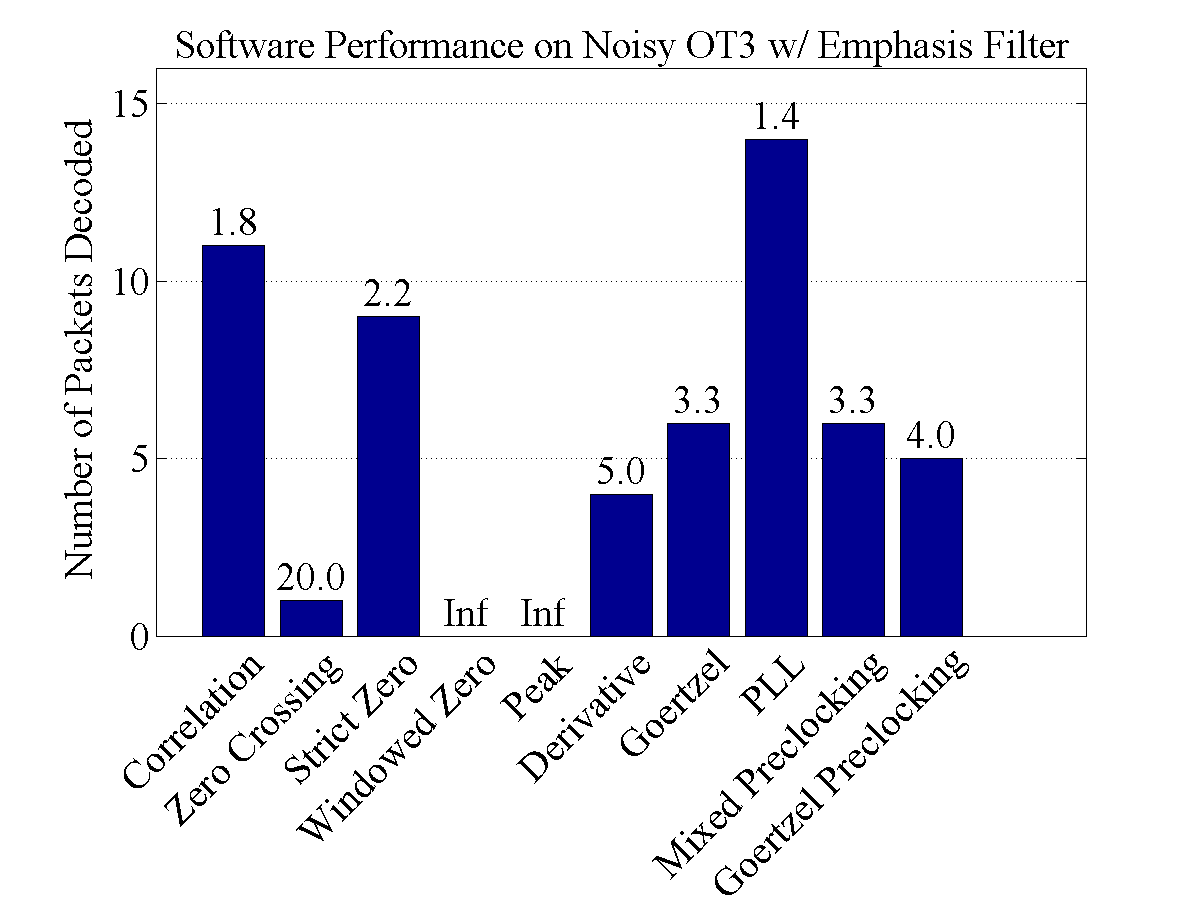
\includegraphics[width=0.75\linewidth]{images/SoftwarePerformanceonNoisyOT3wEmphasisFilter.png} 
	\caption{Performance of Software on OpenTracker Test with noise added with an emphasis filter.}
   \label{OTNoiseFilt6}
\end{figure}

As mentioned earlier, these next two test files were those that were thought the be most important to succeed at. As such, Track 1 was used to tune the algorithms since this would represent the closest real-world simulation possible. The Track 2 results are also presented for comparison. However in Track 2, in addition to being deemphasized the process of this filtering also reduced the magnitude of the signal in the audio file. As such, this file shows two things: One, the ability to pick up lower level signal and second, the algorithms tolerance to signals that were not emphasized when transmitted, but were deemphasized when received. The results of no filtering, bandpass filtering, and emphasis filtering can be seen in their respective Figure \ref{T1FiltNo}, \ref{T1Filt0}, and \ref{T1Filt6} for Track 1. The data from demodulating Track 2 can be seen in Figure \ref{T2FiltNo}, \ref{T2Filt0}, and \ref{T2Filt6}. As was caught during the OpenTracker 3 Test with noise it can be noticed that the Goertzel and PLL algorithms are still doing well on Track 1, and also the Mixed preclocking is doing fairly well. With the filter that is applied on Track 1 to create Track 2 it is basically the opposite effect of Toledo's emphasis filter and hence they cancel each other out. This can be seen by looking at the performance of the Goertzel Demodulator which does poorly with both other filterings on Track 2. However, its ability to detect low level signals and this reversal of the emphasis filtering applied makes it end of having comperable results to the just band pass filter on Track 1 - 956 versus 965. 

\begin{figure}
  \centering
	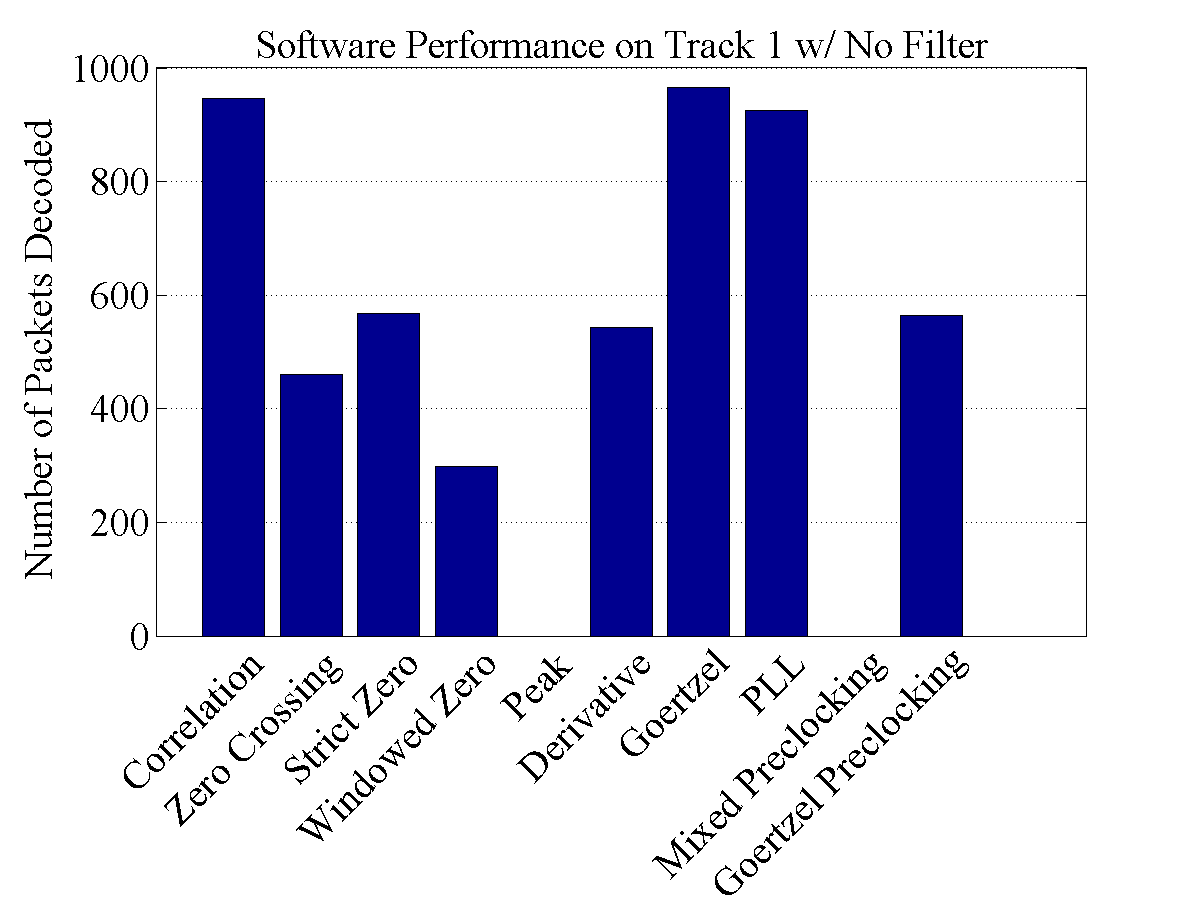
\includegraphics[width=0.75\linewidth]{images/SoftwarePerformanceonTrack1wNoFilter.png} 
	\caption{Performance of software on the raw signal from Track 1.}
   \label{T1FiltNo}
\end{figure}
\begin{figure}
  \centering
	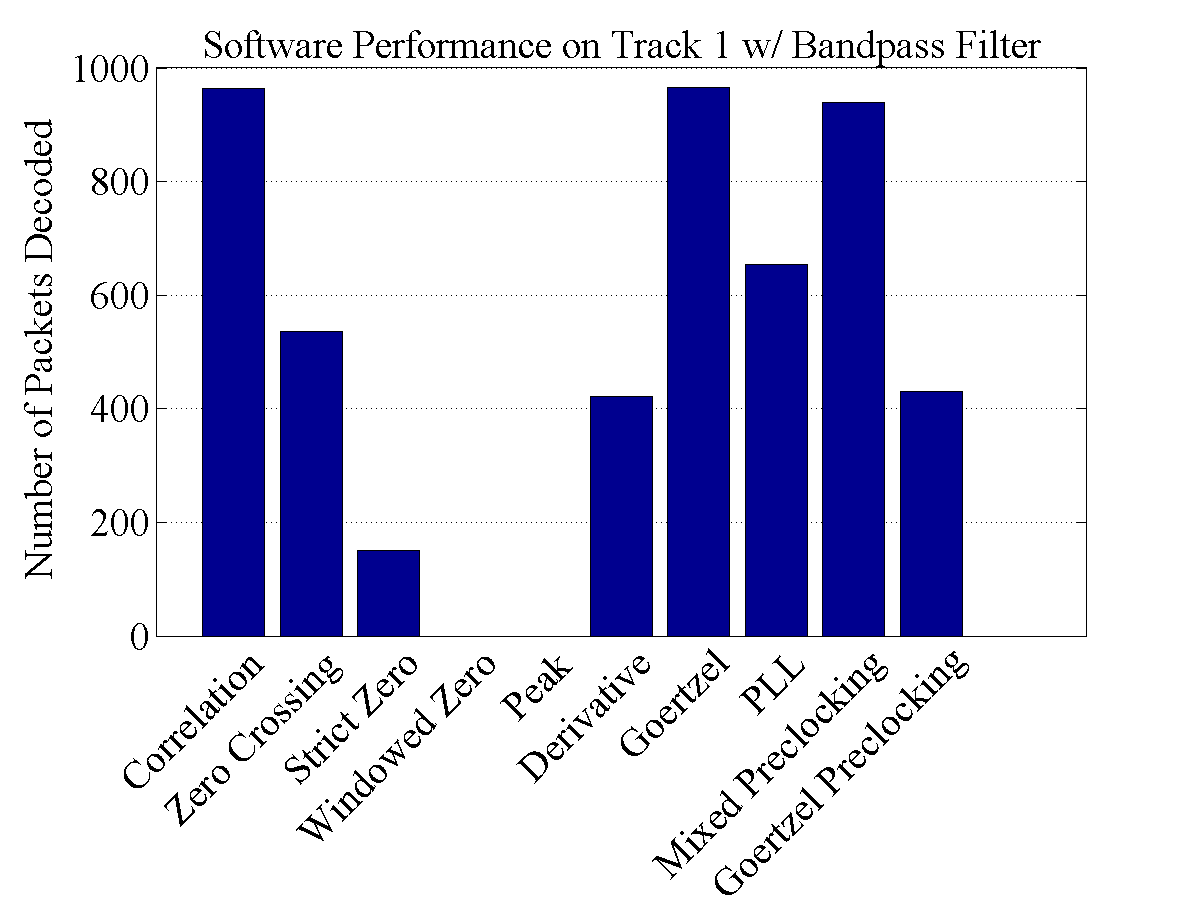
\includegraphics[width=0.75\linewidth]{images/SoftwarePerformanceonTrack1wBandpassFilter.png} 
	\caption{Performance of software on Track 1 with a bandpass filter.}
   \label{T1Filt0}
\end{figure}
\begin{figure}
  \centering
	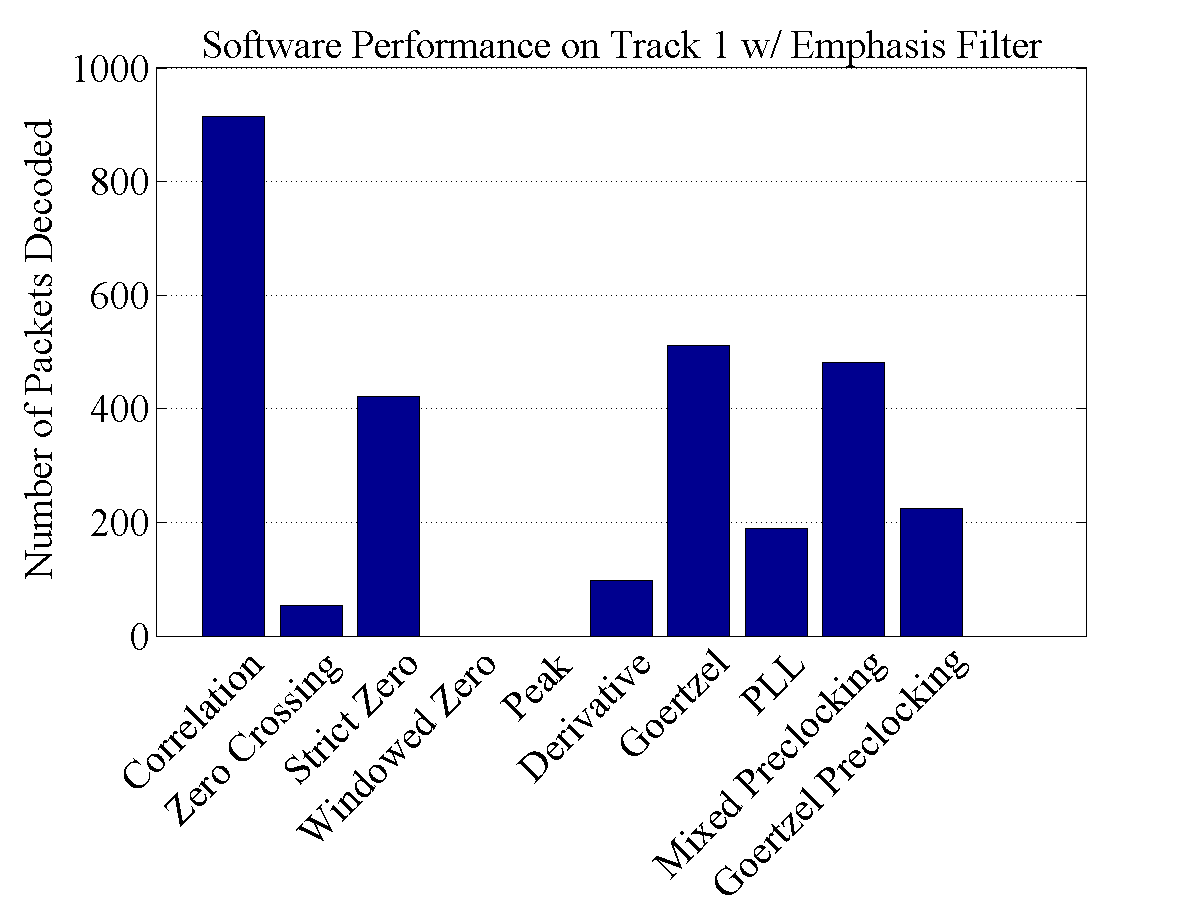
\includegraphics[width=0.75\linewidth]{images/SoftwarePerformanceonTrack1wEmphasisFilter.png} 
	\caption{Performance of software on Track 1 with an emphasis filter.}
   \label{T1Filt6}
\end{figure}
\begin{figure}
  \centering
	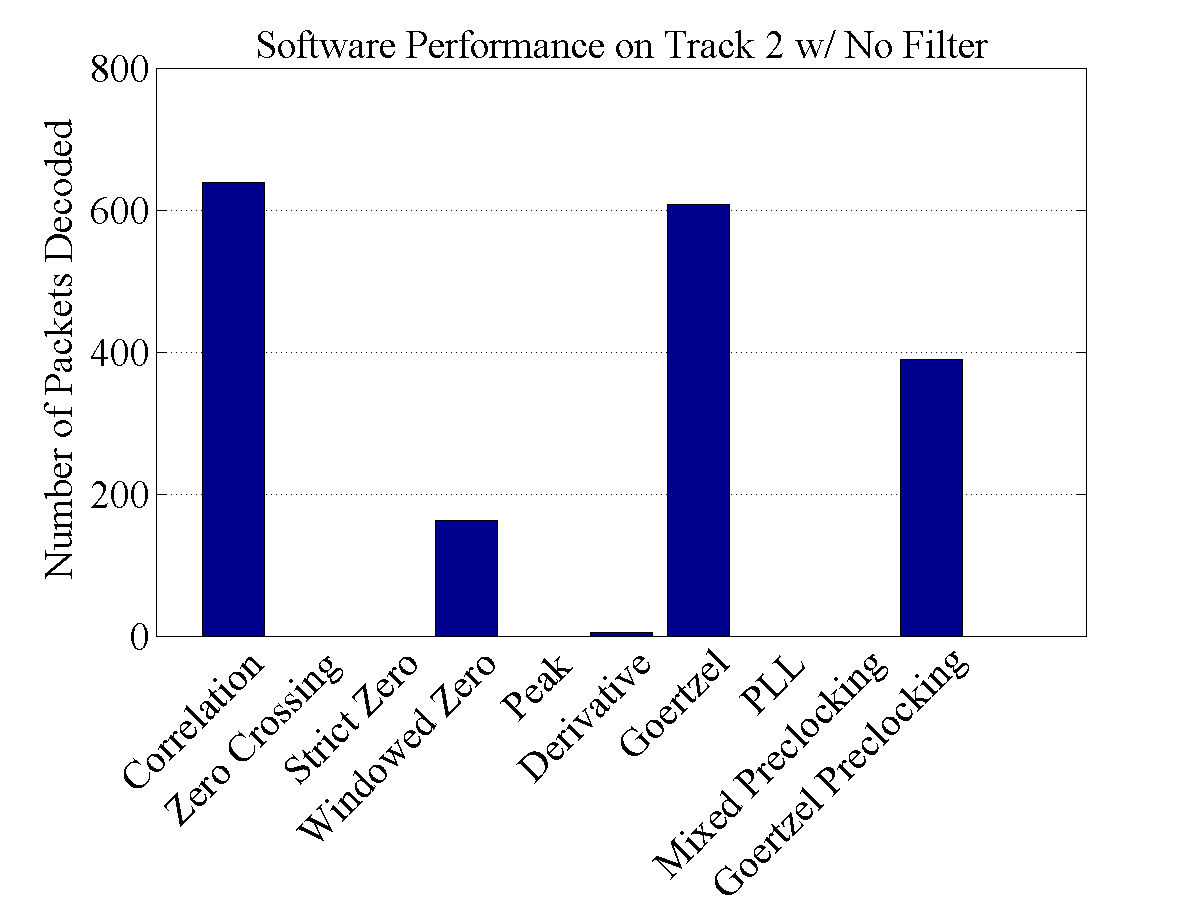
\includegraphics[width=0.75\linewidth]{images/SoftwarePerformanceonTrack2wNoFilter.png} 
	\caption{Performance of software on the raw signal from Track 2.}
   \label{T2FiltNo}
\end{figure}
\begin{figure}
  \centering
	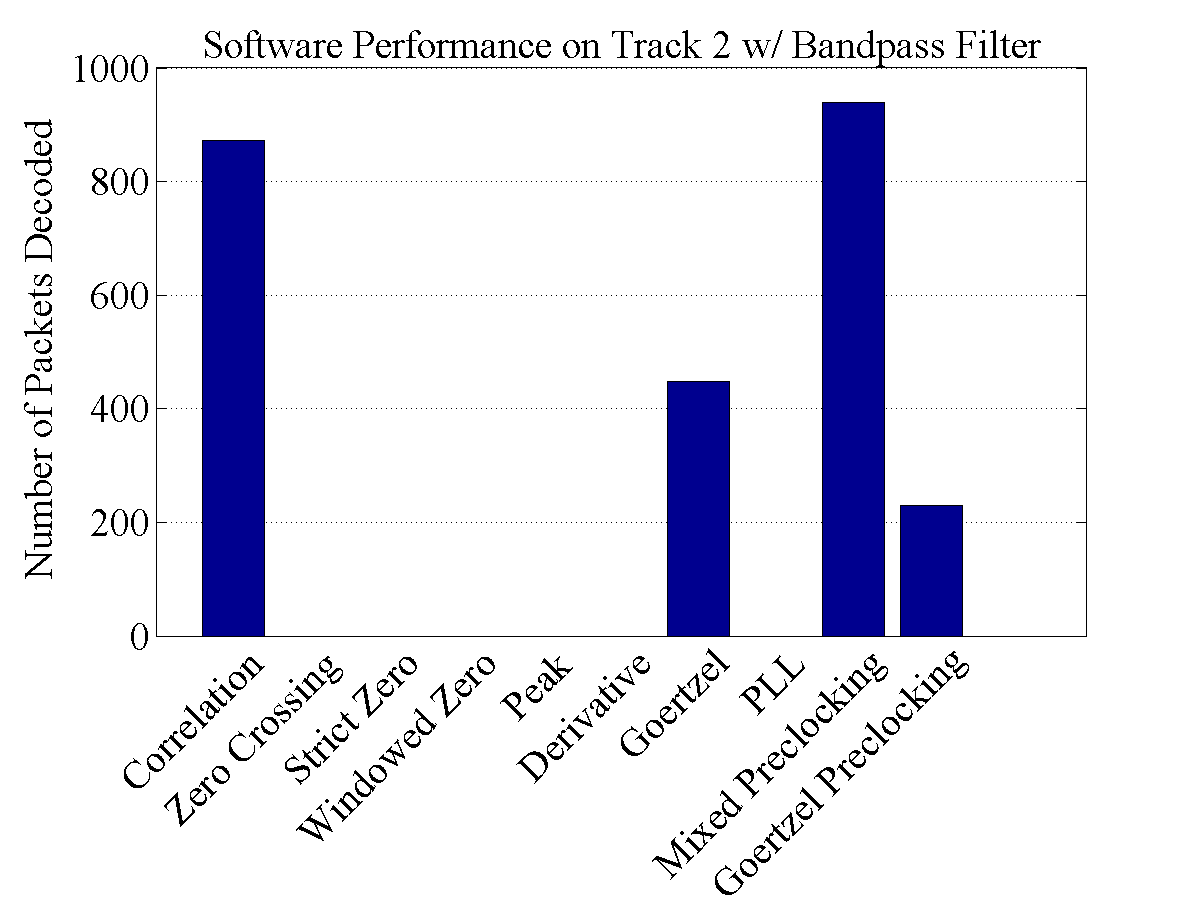
\includegraphics[width=0.75\linewidth]{images/SoftwarePerformanceonTrack2wBandpassFilter.png} 
	\caption{Performance of software on Track 2 with a bandpass filter.}
   \label{T2Filt0}
\end{figure}
\begin{figure}
  \centering
	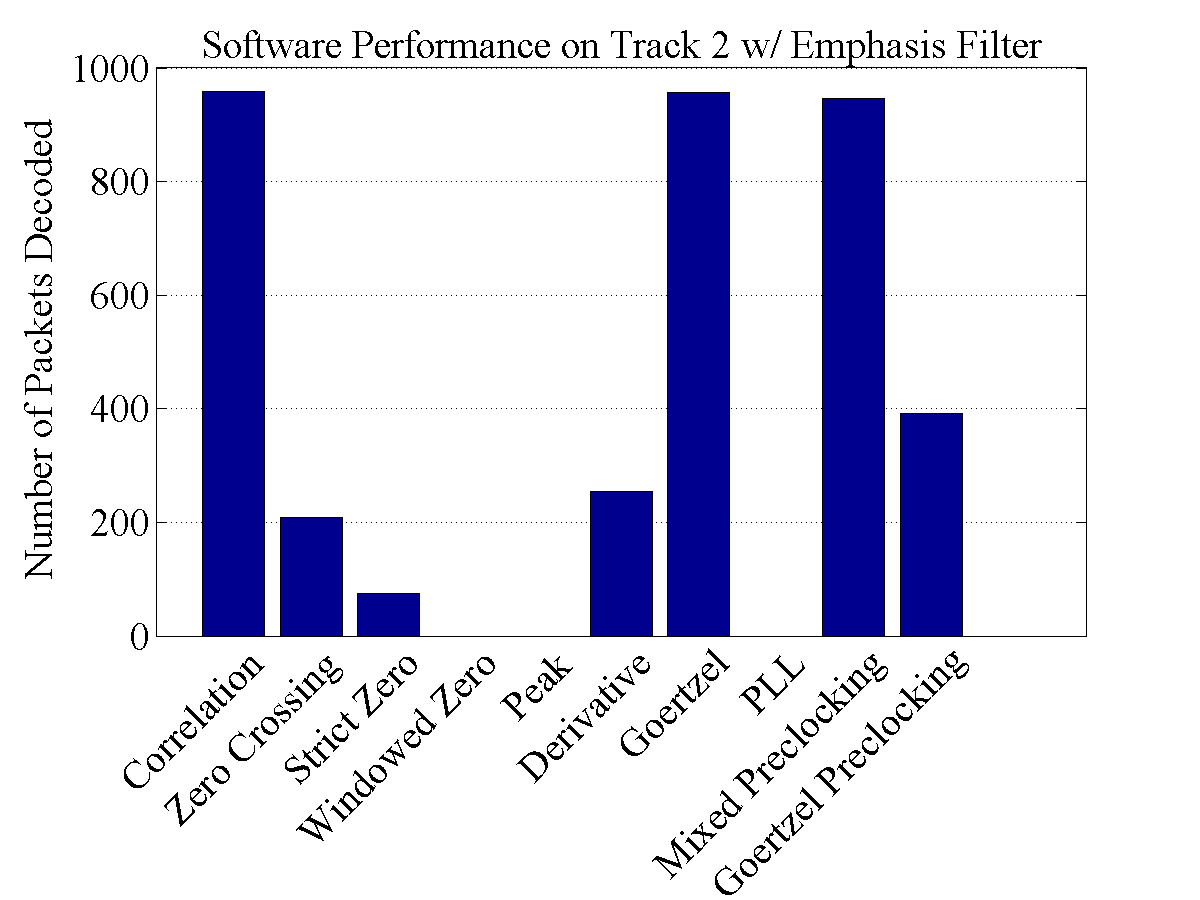
\includegraphics[width=0.75\linewidth]{images/SoftwarePerformanceonTrack2wEmphasisFilter.png} 
	\caption{Performance of software on Track 2 with an emphasis filter.}
   \label{T2Filt6}
\end{figure}


\subsection{Hardware and Software Comparisons}
It is now time to actually compare the new software implementations to the old ones as well as to the hardware. The first thing to notice is that the Goertzel Filter did very well, and in some cases better than the original correlation. Secondly, the complicated preclocking algorithm was also able to hold its own and still be a top contender. In fact the top three software algorithms were Correlation, Goertzel, and Mixed Preclocking with 964, 965, and 939 packets decoded from Track 1 with the bandpass filter. Even though they all have different number of packets decoded they each still have their expertise with being able to exclusively decode packets that others could not. For instance when the three are run together there is a total of 975 packets decoded due to the fact that Goertzel gets 12 packets that the other two do not, Correlation gets 7 that the others do not, and Preclocking decoded 3 that these other two missed. This could still be a good argument for the use of hardware over software since it is very easy to run multiple demodulators in parallel. Especially since the cost of this is only 5 minutes and 2 seconds on a file that is 25:49 long.

The question is, is the software better than the hardware? Looking at the highest numbers, no, but looking at the bigger picture, maybe. One thing about the hardware is that it is prone to variations and in need of periodic tuning. So, if instead of looking at the best of the breed, the average values are compared under the presumption that this would correspond to the average ham's decoding capabilities, then the software does decode more packets. Additionally, the software does not have any capacitors that will dry up or solder joints that may become brittle and affect the performance. The performance of the software today will be exactly the same in 5, 10, many years. The average number of packets decoded by the hardware on Track 1 was 935. Looking at this value any one of the three algorithms that are the top performers would be considered better.

\chapter{Future Work}
The sections in this chapter will explain some aspects that this project uncovered that have the potential for future research. There are three main items that I think should be explored in more depth as future work in this area of AX.25 software based demodulation, they are the discrete Short-Time Fourier Transform, the use of the checksum for forward error correction, and to actually integrate these demodulators with live traffic from a radio.

\section{The Discrete Short-Time Fourier Transform}
In a paper by Zhonghui-Chen et. al. methods are outlined to use the discrete short-time Fourier transform (DSTFT) to demodulate a binary frequency shift keyed (BFSK) signal. After a discussion of the DSTFT they go into their specific implementation, but this appears to show promise because of there results section. Granted this was for a simulation buy they showed that the error rate was lower using the DFTFT than traditional coherent demodulation even for lower signal to noise ratios \cite{Chen2008}

\section{Use the CRC for FEC}
Each AX.25 packet contains a checksum that is generated by using a cyclic redundancy check (CRC). This is used by all demodulators in order to determine if the packet that the demodulator thinks it decoded was actually a legitimate packet or just noise that happened to look like a packet. Although the CRC was not intended for forward error correction (FEC), it would be interesting to see the effects of using it as such. With algorithms such as the Goertzel algorithm the power of each symbol is determined and this power could be used to assign a level of confidence on that demodulated bit. If a packet fails the CRC check, but all except for one of the bits has a confidence greater than 80 percent, would the CRC pass if that one bit was flipped to the other symbol? This is a very good argument for the use of software since this meta data about the decoding of the packets can be kept in memory, something that most hardware is very light on. 

\section{Integrations with a Radio}
Finally another area for future work would be to integrate the new algorithms with a radio and use them to decode live data. Although the data used in the testing was a recording of live data, it would be very gratifying to be able to see these algorithms decode audio straight from the radio. Inside of javaAX25 the packages should already support it, so it should be a matter of just setting it up and letting it run. This analysis would allow for verification of the implementations functionalities as well as to be able to see how the different algorithms perform side by side in real time.


\chapter{Conclusion}
This research set out to try and prove that software could do AX.25 demodulation better than the hardware. Depending on perspective, it may have done so. However, at the very least the research shows that there are many ways to approach the challenge of demodulating these packets and presents the relative performance of over 10 software based approaches and 12 dedicated hardware approaches, whether that hardware is an OpenTracker or TNC.

In the end, the software did do better than the average result using hardware, but in the primary benchmarking file, software was only able to decode 975 packets as opposed to the 1007 that the best piece of hardware detected. Exploring some of the items in the future work section such as using the checksum for forward error correction may be able to get software to the same level as hardware, as it is close.

\bibliographystyle{plain}
\bibliography{../references}

\end{document}
